\documentclass[11pt, a4paper, oneside]{Thesis} 
\usepackage{floatrow}
\floatsetup[table]{capposition=bottom}
\usepackage{textcomp}
\usepackage{wrapfig}
\usepackage{lscape}
\usepackage{rotating}
\usepackage{graphicx, subfigure}
\usepackage{caption}
\usepackage{amsmath}
\usepackage{upgreek}
\usepackage{gensymb}
\usepackage{csquotes}
\usepackage{pdfpages}
\usepackage{lipsum}  
\usepackage{acronym}
\usepackage{array}
\newcolumntype{L}{>{\centering\arraybackslash}m{3cm}}
\usepackage{apacite}
%\usepackage{natbib}
\bibliographystyle{apacite} % Use the "custom" BibTeX style for formatting the Bibliography




\makeatletter
\AtBeginDocument{%
  \renewcommand*{\AC@hyperlink}[2]{%
    \begingroup
      \hypersetup{hidelinks}%
      \hyperlink{#1}{#2}%
    \endgroup
  }%
}
\makeatother


\graphicspath{{Images/}} 
%\usepackage[square, numbers]{natbib} % Use the natbib reference package - read up on this to edit the reference style; if you want text (e.g. Smith et al., 2012) for the in-text references (instead of numbers), remove 'numbers' v
\hypersetup{urlcolor=black, colorlinks=true} 
\title{\ttitle} 
\begin{document}
\makeatletter
\renewcommand*{\NAT@nmfmt}[1]{\textsc{#1}}
\makeatother
\frontmatter
\setstretch{1.6} 
\fancyhead{} 
\rhead{\thepage}
\lhead{}
\pagestyle{fancy} 

\newcommand{\HRule}{\rule{\linewidth}{0.5mm}} 
% PDF meta-data
\hypersetup{pdftitle={\ttitle}}
\hypersetup{pdfsubject=\subjectname}
\hypersetup{pdfauthor=\authornames}
\hypersetup{pdfkeywords=\keywordnames}

%\captionsetup[figure]{labelfont={bf},name={Figure},labelsep=period}
\captionsetup[figure]{labelfont={bf},name={Figure}}
\captionsetup[table]{labelfont={bf}, name = {Table}}
\captionsetup[table]{position=bottom} 

\begin{titlepage}
\begin{center}

\HRule \\[0.4cm] % Horizontal line
{\huge \bfseries \ttitle}\\[0.4cm] % Thesis title
\HRule \\[1.5cm] % Horizontal line
 
\large \textit{A thesis submitted in fulfilment of the requirements\\ for the degree of \degreename}\\[0.3cm] % University requirement text
\textit{by}\\[0.4cm]
\authornames \\
20128405 \\ [0.4cm]



\vfill
\graphicspath{ {./Figures/} }
\begin{figure}[hb]
  \centering
  
\includegraphics[width=0.35\linewidth]{Images/iitk_logo.png}
\end{figure}

\DEPTNAME\\ % Research group name and department name
\textsc{ \UNIVNAME}\\[1.5cm] % University name
\large \today\\[2cm] % Date

\end{center}

\end{titlepage}

\Declaration{\addtocontents{toc}{\vspace{1em}}}
\setcounter{page}{2}

\begin{minipage}{\textwidth}
    
    It is certified that the work contained in this thesis entitled \textbf{\enquote{\ttitle}} by \textbf{\authornames} has been carried out under my supervision and that it has not been submitted elsewhere for a degree.
        
\end{minipage}

\vspace{20.00mm}

\begin{minipage}{0.49\textwidth}
		\begin{flushleft}
			{\supnameA\\ 
			Associate Professor\\
			\deptname\\
			\univname}
		\end{flushleft}
\end{minipage}

\vspace{2cm}

\begin{center} 
    \today\\[2cm]
\end{center}

\vfill
\clearpage % Start a new page
\StudentDeclaration{\addtocontents{toc}{\vspace{1em}}} % Add a gap in the Contents, for aesthetics

This is to certify that the thesis titled \textbf{``\ttitle''} has been authored by me. It presents the research conducted by me under the supervision of \textbf{\supnameA}.\par

To the best of my knowledge, it is an original work, both in terms of research content and narrative, and has not been submitted elsewhere, in part or in full, for a degree. Further, due credit has been attributed to the relevant state-of-the-art and collaborations with appropriate citations and acknowledgments, in line with established norms and practices.\\ [2cm]
\begin{minipage}{.5\textwidth}
		\begin{flushleft}
			{\authornames\\ Roll No. 20128405 \\
			\normalsize{\href{https://www.cgs.iitk.ac.in/}{CGS Department}\\
			\univname}}
		\end{flushleft}
\end{minipage}
\vfill

\clearpage % Start a new page



\lhead{\emph{Abstract}}
\abstract{\addtocontents{toc}{\vspace{1em}} 
One of the fundamental human abilities involved in human-environment interaction is extending one's arm to make physical contact with an object. To perform a successful reaching action, the agent's cognitive system must encode the spatial location of the target. Peri-personal space is the region of space surrounding the agent's body where reach targets are located. One of the characteristics of peri-personal space is that the objects in this region of space are encoded with respect to the region of the body-surface that is in close proximity to the object. In addition, action-relevant body parameters, such as the position and structure of the limbs, are encoded in a body representation which is constructed by integrating visual and proprioceptive sensory information about the body. 

Considering the above, this thesis investigates the following two questions. Firstly, is the spatial information of the reach target encoded relative to the body part located proximally, even if that body part is not the effector performing the reach action? Secondly, if the answer to the first question is affirmative, how does the integration of visuo-proprioceptive signals regarding the proximal body part contribute to the spatial encoding of the target? To investigate these questions, two  experiments were conducted in an immersive virtual reality set-up, in which a reach task was performed while the action hand was rendered invisible. Visual and proprioceptive information of the proximal body part was manipulated as the experimental conditions, and the accuracy of reaches was measured. The results of the two experiments indicate that the spatial encoding of the reach target occurs relative to the proximal body-part, and that the integration of the proximal body-part's visual and proprioceptive sensory signals underlies the spatial encoding of the reach target's location. However, the results further suggest that the spatial encoding of the target occurs relative to the body-part location indicated by its visual signal, as opposed to the body-part position inferred after the integration of multi-sensory signals.









%Reaching one's arm out to make contact with an object is one of the fundamental human capabilities involved in human-environment interaction. To perform a successful reaching action, the spatial location of the target must be encoded in the cognitive system of the agent. Targets of reach action are located in the region of space surrounding the agent's body- termed as \textit{peri-personal space}. One of the characteristics of peri-personal space is that the objects located in this region of space are encoded with respect to the region of the body-surface which is in proximity to the target. Moreover, body parameters relevant for action, such as position and structure of the limbs, are encoded in a body representation which may be constructed from the integration of visual and proprioceptive sensory information regarding the body. 

%Considering the above, we investigated the following two questions in this thesis. Firstly, is the spatial information of the reach target encoded with respect to the body-part situated in its proximity, even if that body-part is not the effector undertaking the reach action? Secondly, if yes, how is the integration of visuo-proprioceptive signals regarding the proximal body-part involved in the spatial encoding of the target? To investigate these questions, two experiments were conducted in an immersive virtual reality environment, in which a reach task was implemented while the action hand was rendered invisible. Visual and proprioceptive information of the proximal body-part were also manipulated as the experimental conditions, and the accuracy of the reaches was measured. The results of the two experiments suggest that the spatial encoding of the reach target occurs with respect to the proximal body-part, and that integration of proximal body-part's visual and proprioceptive sensory signals underlies the encoding of the reach target's spatial location. However, the results further suggest that the spatial encoding of the target occurs with respect to the body-part location indicated by its visual signal as opposed to the body-part location estimated as a result of multi-sensory integration process.

}
\clearpage 
\setstretch{1.3} % Reset the line-spacing to 1.3 for body text (if it has changed)

\acknowledgements{\addtocontents{toc}{\vspace{1em}} % Add a gap in the Contents, for aesthetics

From bottom of my heart, I offer gratitude to the following people, who have been instrumental in bringing this work into existence.

To Prof. Devpriya Kumar, my supervisor, for the unwavering patience in guidance and answering every little question of mine, teaching me everything I know today about research, and cracking cringe-worthy jokes that have mostly succeeded in keeping my spirits up!

To Saee and Roshan, for the memes and laughter, for the long hours of conversations and hang-outs, and for the unparalleled emotional support!

To my colleagues in the lab and the department- Aditi, Rujuta, Arjun, Revati, Ishan, Hariharan, Shivani, Anjali, and others- for  being present to listen to my thoughts, ideas, and questions, and always ending the conversation with a variant of "Ho Jaayega"! 

To Mummy and Pappa, for making sure that I'm eating properly, even from a thousand kilometers away!

And lastly, to Butterscotch, Brownie, and Caramel, for joining me for chai and biscuits for many of my evenings, never hesitating to show affection through jumps, barks, and a lot of dog-hair left on my clothes.


}
\clearpage % Start a new page
\pagestyle{fancy} % The page style headers have been "empty" all this time, now use the "fancy" headers as defined before to bring them back

\lhead{\emph{Contents}} % Set the left side page header to "Contents"
\tableofcontents % Write out the Table of Contents

\lhead{\emph{List of Figures}} % Set the left side page header to "List of Figures"
\listoffigures % Write out the List of Figures

\lhead{\emph{List of Tables}} % Set the left side page header to "List of Tables"
\listoftables % Write out the List of Tables



\clearpage 
\setstretch{1.5} 
\lhead{\emph{Abbreviations}} 

%\chapter*{Abbreviations}
%\addtotoc{Abbreviations}
%\begin{acronym}[XXXXXXXXX] % Give the longest label here so that the list is nicely aligned
\acro{PPS}{Peri-Personal Space}
\acro{PHT}{Distance between the actual position of the hand and visual rendering of the hand in Experiment 2}


\end{acronym}

\clearpage 
\setstretch{1.3} 
\pagestyle{empty} 
\dedicatory{Dedicated to my Guru, Dr. Vishnu Ramachandra Parnerkar} % Dedication text
\addtocontents{toc}{\vspace{2em}} 

%	THESIS CONTENT - CHAPTERS

\mainmatter
\pagestyle{fancy} 

\chapter{Introduction} 
\label{introduction} 
\lhead{Chapter 1. \emph{Introduction}} 


You extend your arm to grab a cup of coffee, grasp the book you're holding, or swat a mosquito buzzing around your ears. One of the most common ways we interact with our surroundings is by reaching out with our hands to touch the objects in our surroundings. Reaching is one of the fundamental human actions involved in human-environment interaction, underpinning diverse abilities such as feeding, object manipulation, and self-defense. A characteristic feature of reaching action is that it is goal-directed towards a specific external target. Once the target is specified during the action selection stage, it must be translated into a movement plan so that the effector (the hand) can make contact with the target(eg. the coffee mug). To accomplish this, \textit{the spatial location} of the coffee mug must be encoded in a format suitable for motor control. Information from various sensory modalities about the spatial location of the target have to be integrated with the spatial information of the effector to perform an accurate reach. How is the spatial information of the reach target encoded? In particular, what is the reference frame in which the reach target is spatially encoded? 

%You reach your arm out to grab a cup of coffee, to grasp the book in your hand, or to swat off the mosquito buzzing around your ears.  One of the most common ways we interact with the environment is through reaching out our hands in order to make contact with the objects in our environment. Reaching action is one of the fundamental human actions involved in human-environment interaction, underlying various capabilities like feeding, object manipulation, or self-defense. A characteristic of reaching action is that it is goal directed towards a specific target in the external environment. Once the target is specified in the action selection stage, this goal must be transformed into a movement plan, so that the effector (the hand) can make contact with the target (the coffee cup). For this purpose, the spatial location of the cup of coffee must be encoded, in a format appropriate for motor control. Information from various sensory modalities about the spatial location of the target have to be integrated with the spatial information of the effector to perform an accurate reach. How is the spatial information of the reach target encoded? In particular, what is the reference frame in which the reach target is spatially encoded? 

%The region of space immediately surrounding the body is termed as peri-personal space. A distinction is made between peri-personal space and extra-personal space, because of certain behavioural and neuro-physiological effects observed when objects are present in peri-personal space. For instance, 

The targets of reaching action are situated in the region of in close proximity to the body, which is termed in the literature as \emph{peri-personal space}. The characteristic feature of representation of spatial information of objects in peri-personal space is that it is encoded with respect to the area of body which is in proximity to the object \cite{serino2019peripersonal}.
 This notion that the representation of spatial information of the object is "anchored" to the proximal body-part is supported by both neuro-physiological and behavioural evidence (See Chapter \ref{Literature Review}). For instance, visuo-tactile multi-sensory interaction effects such as the \emph{cross-modal congruency effect} has been observed in certain experiments, wherein subjects localize tactile stimuli faster when a task-irrelevant visual cue is presented congruent to that body part, as compared to the condition where the task irrelevant cue is presented incongruent to the tactile stimulated body part \cite{spence2004multisensory}. The magnitude of cross-modal congruency effect (and other similar multi-sensory interaction effects) is also indicative of the distance between the stimuli and the body \cite{spence2004spatial, iachini2014motor}, that is, these multi-sensory responses increase as the distance between the visual stimuli and the body decreases. 
 
 %These results are indicative of two notions - i) Visual objects in peri-personal space are spatially with respect to the proximal body-part, and ii) Multi-sensory 

 These multi-sensory interaction effects are used in literature as a proxy for understanding how peri-personal space in implicated in various cognitive processes. For instance, a functional link has been demonstrated between action and multi-sensory behavioural responses evoked by objects in peri-personal space \cite{ladavas2008action, patane2019action, brozzoli2010action}, suggesting that the peri-personal space representation serves as a perceptual-motor interface for guiding goal directed actions. Furthermore, the multi-sensory interaction effects are also modulated by action possibilities \cite{lohmann2019hands, iriki1996coding, senna2019aim}. It has thus been theorized that a generative mechanism underlies representation of peri-personal space, which predicts the likelihood of future sensory outcomes \cite{lohmann2019hands, noel2018peri}. In this light, the representation of spatial information of objects in peri-personal space could be interpreted as a representation of space in terms of a constantly updated set of probabilities that carry information about the likelihood that stimuli in the space around the body will make contact with a specific area of the body. If this is indeed the case, modulating parameters that affect the representation of peri-personal space should affect the outcome of actions involving contact, that is, reaching actions. However, one of the gaps in the literature is that the link between goal directed action and peri-personal space- where the reach action targets are present, has only been investigated through the multi-sensory interaction effects paradigm, and not through the outcome of reach action- that is, how accurate were the subjects in estimating the location of the target, when factors affecting peri-personal space representations are modulated.

 If the reach targets are spatially encoded with respect to body-part proximal to them, it is plausible that the representation of body parameters is also involved in the reach targets' spatial encoding. One of the views in the literature is that the cognitive system represents body parameters, particularly those necessary for motor control- including the spatial information of the effector, in an integrated representation termed as \emph{body schema} \cite{ataria2021body}. Notably, the construction of body schema is commonly conceptualized as an inference problem, where most probable estimates of the body parameters (here, the spatial position of the body-part) are dynamically computed from the inflow of sensory inputs from various sensory modalities, like vision and proprioception \cite{van1999integration}. In other words, a visuo-proprioceptive integrative mechanism underlies the specification of spatial information in body schema. Could the same visuo-proprioceptive integration mechanism which specifies the spatial information of the body-part, also underlie the spatial encoding of the reach target which lies in proximity to this body-part?

 To investigate this question, two experiments were conducted in which a reaching action task paradigm was implemented in an immersive virtual reality environment. With their action hands rendered invisible, the subjects were asked to make contact with a visual target, while visual and proprioceptive information of the action-irrelevant body part proximal to the target was manipulated, and accuracy of target location estimated by the participant was measured. In the first experiment, we investigated whether the reach target location estimation is indeed affected by the presence or absence of a proximal body-part, and if so, how does the uni-sensory and multi-sensory information of the proximal body-part affect the reach target location estimation. In the second experiment, we attempted to probe further into how visuo-proprioceptive integration mechanism underlies the spatial encoding of reach target, by manipulating the spatial discrepancies between the visual and proprioceptive information of the proximal body-part. The results of the two experiments support the hypothesis that reach target is encoded with respect to the proximal body-part, and that its multi-sensory integration mechanism underlies the reach action target encoding. However, the results suggest that the spatial encoding of reach target occurs relative to the location specified by the visual information of the proximal body-part, as opposed to the location of the body-part inferred after the multi-sensory integration process.


 

 %The objective of this thesis is to understand how the integration of visuo-proprioceptive information regarding the body in proximity to the reach action target underlies the encoding of its spatial information. To investigate this question, two experiments were conducted. In both experiments, a reaching action task was implemented in an immersive virtual environment, in which the subjects were asked to make contact with a target, with their action hand rendered invisible. The visual and proprioceptive information of a body-part which is in proximity to the target, but not directly relevant to the task of reaching action, was manipulated, while the end point of the reaching action was measured as the subject's estimated target location. We expected that the discrepancies between the spatial estimates provided by visual and proprioceptive input regarding the position of the proximal body-part should affect the spatial representation of the target, which should be observable in the estimation of target location in the reaching action. The aim of the first experiment was to seek empirical evidence supporting the notion that spatial encoding of target is affected by sensory information regarding the body-part which is in proximity to it, by investigating the differences in the target location estimation accuracy between visual and proprioceptive uni-sensory and multi-sensory inputs of the proximal body-part.  In the second experiment, we probed further into the integration mechanism by inducing systematic spatial discrepancies between the visual and proprioceptive inputs to understand its effect on the target location estimation. Based on the results of the two experiments, we find evidence suggesting that the sensory inputs about the proximal body-part does indeed underlie the spatial encoding of the reach target. Furthermore, the spatial representation seems to be predominantly anchored to the visual information of the proximal body part. However, the integration of the visual input with proprioception may be necessary for the the anchoring to occur more accurately.


%One of the views in the literature is that the cognitive system represents body parameters essential for motor control, including the spatial information of the effector, in an integrated representation termed as \emph{body schema} \cite{ataria2021body}. The construction of body schema is commonly conceptualized as an inference problem, where most probable estimates of the body parameters are dynamically computed from the inflow of sensory inputs from various sensory modalities, like vision and proprioception \cite{van1999integration}, on the basis of the reliability of the sensory input (noise), and the prior beliefs encoded in the system regarding the relevance of the sensory inputs. Thus, a visuo-proprioceptive integrative mechanism underlies the specification of spatial information in body schema, which is utilized for planning and guiding the reaching action.


%Thus, body-part anchoring and body-object proximity dependence are two important properties associated with how the spatial information of objects in peri-personal space is represented. Moreover, contact-location prediction in goal-directed action is one of the functional explanation to the nature of peri-personal space representation. Thus, the two properties of spatial encoding of objects - the body-part anchoring and the body-object proximity dependence, should also be involved in the outcome of actions involving contact. The body-part anchoring also suggests that not only does the representation of bodily parameters specified in body schema provide information about the state of the effector, but that body schema may also be involved in spatial encoding of action target and specifying the target's spatial location with respect to the body. Since visuo-proprioceptive integrative mechanisms underlie construction of body schema, disturbances in the multi-sensory integration process should affect the spatial encoding of the target in its proximity. Therefore, visuo-proprioceptive discrepancies in the body-part proximal to the target should affect the estimation of target location in reaching action.

%To investigate this conjecture, a reaching action task was implemented in an immersive virtual environment, in which visual and proprioceptive information of a body-part which is in proximity to the target, but not directly relevant to the task of reaching action, was manipulated. We expected that the visuo-proprioceptive discrepancies of the body should affect the spatial representation of the target, which should be observable in the estimation of target location in the reaching action.

%The objective of this thesis is to understand how the integration of visuo-proprioceptive information regarding the body in proximity to the reach action target underlies the encoding of its spatial information. To investigate this question, two experiments were conducted. In both experiments, a reaching action task was implemented in an immersive virtual environment, in which the subjects were asked to make contact with a target, with their action hand rendered invisible. The visual and proprioceptive information of a body-part which is in proximity to the target, but not directly relevant to the task of reaching action, was manipulated, while the end point of the reaching action was measured as the subject's estimated target location. We expected that the discrepancies between the spatial estimates provided by visual and proprioceptive input regarding the position of the proximal body-part should affect the spatial representation of the target, which should be observable in the estimation of target location in the reaching action. The aim of the first experiment was to seek empirical evidence supporting the notion that spatial encoding of target is affected by sensory information regarding the body-part which is in proximity to it, by investigating the differences in the target location estimation accuracy between visual and proprioceptive uni-sensory and multi-sensory inputs of the proximal body-part.  In the second experiment, we probed further into the integration mechanism by inducing systematic spatial discrepancies between the visual and proprioceptive inputs to understand its effect on the target location estimation. Based on the results of the two experiments, we find evidence suggesting that the sensory inputs about the proximal body-part does indeed underlie the spatial encoding of the reach target. Furthermore, the spatial representation seems to be predominantly anchored to the visual information of the proximal body part. However, the integration of the visual input with proprioception may be necessary for the the anchoring to occur more accurately.


\chapter{Literature review} 
\label{Literature Review} 
\lhead{Chapter 2. \emph{Literature Review}} 

One of the classic questions in the philosophy of cognition is - What is the relationship between perception and action? One of the dominant ideas is that the purpose of perception is to gather information for guiding action, while action is a means to acquire perceptual information regarding the environment. In reaching action, action is directed towards objects of interest in the external environment. The body is central to the process of reaching action. Not only is the reach carried out by bodily movements, but the targets of reaching actions also lie in space close to the body(peri-personal space). Thus, for a reaching action, the cognitive system of the agent requires i) knowledge of body for computing the state of the effector (the body entity with which the action is carried out), and ii) information regarding the object of interest (the target entity on which the action is carried upon). Perceptual processes provide knowledge to the system regarding both these entities.

The aim of this chapter is to provide relevant background and discuss key concepts, theories and empirical findings that led to the development of the conjecture that we have investigated in this thesis. This chapter will thus be divided into two parts - the body and the target. Part I consists of a brief discussion on body representation, and its role in motor control. In Part II, we delve into theories and findings regarding peri-personal space, where the reach action target lies, and its implications in unfolding of action. I will end with connecting these distinct strands of literature and stating the conjecture. 


\section{Body representation and Action}

Goal-directed action require information about properties of one's body, in order to plan movements, and guide the action. These properties include both structural and positional parameters of the body. Precise position of one's limbs, not only during action initiation (t = 0), but also during the action execution, is an important parameter for a successful action. Furthermore, information regarding structural properties of one's body, such as body configuration, body size, flexibility of joints, muscle strength, are necessary so that movements do not occur in biologically impossible or painful manner. According to the review by \citeA{ataria2021body}, one of the claims in the literature is that the cognitive system of the agent represents the above mentioned properties in an integrated representation of the body, termed as \emph{body schema}. Importantly, body schema is conceptually distinguished from other body representations like body image, by the notion that the parameters encoded in body schema are in a specific format. Evidence from \citeA{schwoebel2005evidence}'s study suggests that body parameters are encoded in three distinct representational formats - sensorimotor, visuo-spatial, and linguistic. Body schema encodes the bodily parameters in a sensorimotor format, which the motor system can directly exploit.

In the control-theoretic model of action, two types of process models have been proposed- the inverse model and the forward model, both of which function parallelly. The claim is that body schema plays a role in both these processes. The inverse model computes the motor commands required to achieve the goal, or the final state of the action, constrained by the current body capacities, which are represented in the body schema.  The forward model predicts sensorimotor consequences of the action \cite{wolpert2001motor}. Here, the execution of action is guided by matching the anticipatory model of the body, with the current model of the body, as represented by the body schema. \citeA{ataria2021body} thus proposes a dual function of body schema - description of the body at a spatial resolution and format which can be utilized by the motor system, and for the anticipatory control of action.

\subsection{Construction of body schema}

One of the dominant questions regarding the body schema is -  what are the computations underlying the construction of body schema. \citeA{ataria2021body} suggests that construction of body schema is a dynamic process, that is, the body representation is continuously updated to adapt to the bodily changes throughout development and other short term changes like changes in environment, ill-health, pregnancy, or tool use. 

One of the theories for understanding the construction of body schema is that the generation of body schema can be thought of as an inference problem, to compute the most reliable estimates of body parameters from the inflow of sensory inputs from various sensory modalities, like vision and proprioception \cite{van1999integration}. The Bayesian model of multi-sensory integration proposes that the cognitive system computes the most probable output, here, the parameters specifying the body schema, from the sensory cues available, on the basis of the reliability of the sensory cues (noise), and the prior beliefs encoded in the system regarding the relevance of the cues.  In a novel bodily situation, online sensory cues will be favoured, versus the beliefs regarding the past body representations. Furthermore, the success of action also informs the construction of the body schema. If the action is successful, the process underlying the generation of body schema is confirmed, whereas, if the action is unsuccessful, the body schema needs to be updated for future actions. Thus, Bayesian view provides a description of how body schema is dynamically constructed. 

 Furthermore, the role of integration of inputs from multiple modalities in demonstrating the plasticity of the body representation has also been empirically demonstrated through the Rubber Hand Illusion. In this paradigm, when a rubber hand is stroked synchronously with a participant's unseen real hand, they tend to i) perceive the location of their hand as displaced towards the rubber hand \cite{tsakiris2005rubber} , ii) perceive tactile sensation through the rubber hand \cite{pavani2000visual}, and iii) experience a feeling of ownership over the rubber hand \cite{longo2008embodiment}.  

 There are two major challenges regarding the computations of the multi-sensory integration processes underlying the emergence of body schema. The first is how to identify and select which are the relevant sensory signals to bind together- a problem termed as the "parsing problem". The second problem is, once the relevant signals are selected, how are the signals integrated into a coherent body representation? Every sensory signal is encoded in a different modality-specific format, and in a particular frame of reference, which needs to be resolved into a common format and reference frame. Furthermore, different sensory cues are assigned different weights based on their reliability and relevance. How are these weights assigned, is an important question to consider.

Summarizing this section, body schema specifies bodily parameters which are relevant for action planning and control, and the construction of body schema is a dynamic process relying on a process of multi-sensory integration of sensory inputs from vision and proprioception. We will now turn towards a discussion regarding perception of the action target and the representation of its spatial location.

 \section{Peri-personal space}

 \begin{figure}
\centering    
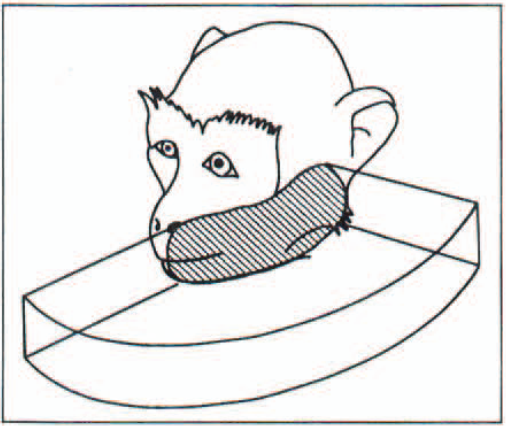
\includegraphics[width=70mm]{Images/bimodal.png}
\caption{Spatially corresponding tactile receptive field (striped) and visual receptive field (boxed) of a bimodal neuron in putamen \citep{graziano1994mapping}}
\label{fig:bimodal}
\end{figure}

 In the cognitive system, the representation of space provides a framework regarding how different objects in the external environment are located with respect to each other, and with respect to the self. Other than abstract and geographical spatial representations, the prominent characteristic of space representation is that body, or a body-part is the origin of spatial representations. Spatial information is processed in several reference frames, depending on the sensory source of the information and the agent environment interaction. For example, the spatial location of an approaching bee will be processed not only in eye-centered and head-centered reference frames due to visual and auditory inputs, but also in reference to the hand to which it is approaching to avoid getting strung \cite{serino2019peripersonal}. However, exponentially, the agent does not have explicit access to these distinct representations, suggesting integration of different reference frames into a unified global reference frame (as reviewed by \citeA{serino2019peripersonal}). 

Peri-personal space is the region of space in close proximity to the body. Its representation is distinct from the representations of extra-personal space (regions of space far from the body), based on findings from lesion studies in monkeys that show that different neuronal populations encode peri-personal and extra-personal space \cite{rizzolatti1983deficits}.

%Peri-personal space is relevant for this work because the target of reach actions lie in the peri-personal space. For the purpose of this thesis, it is thus helpful to think of peri-personal space representations in terms of representing the distance of the object from the part of body in its proximity. 
 
\subsection{Objects in peri-personal space are represented with respect to the body-part in proximity}

The spatial location of objects in peri-personal space is represented by an underlying multi-sensory mechanism. This notion is supported by both neurophysiological studies in macaque monkeys and behavioural studies in humans. Results from primate studies show evidence of bimodal neurons in several regions of the brain - premotor cortex, putamen, and parietal area 7B \cite{graziano1994mapping}. These neurons have visual and tactile receptive fields which spatially correspond with each other (refer Figure \ref{fig:bimodal}), and respond to both visual and tactile stimuli, when they are present in their respective receptive fields.
Furthermore, evidence from \citeA{avillac2007multisensory} is also indicative of neural computation of multi-sensory integration, where evoked multi-sensory responses are either sub-additive or super-additive than than sum of uni-modal responses. This dual receptive field property of these bimodal neurons is not just indicative of the multi-sensory mechanisms underlying peri-personal space representation, but also that these bimodal neurons integrate the visual signal with the location of the body near which the visual stimulus appears, suggesting that the representation of the spatial location of the objects is anchored to the surface of the body in the object's proximity.

The body-part centered representation of peri-personal space is also supported by multi-sensory interaction effects demonstrated in human behavioural studies. Results from cross-modal congruency effect experiments show that participants localize tactile stimulation faster when a task-irrelevant visual cue is presented congruent to that body part, as compared to the condition where the task irrelevant cue is presented incongruent to the tactile stimulated body part \cite{spence2004multisensory}. Similarly, participants are quicker in responding to tactile stimulation where task-irrelevant visual cue is present, compared to the condition where visual cue is absent \cite{patane2019action}. Furthermore, these multi-sensory effects are dependent on the distance of the visual stimuli to the body, as evidenced by the finding that the magnitude of multi-sensory interactions is greater in regions of space near the body as compared to far away from the body \cite{spence2004spatial}, and processing times of stimuli in peri-personal space is faster as compared to extra-personal space \cite{iachini2014motor}. Consequently, these effects are used as measures for peri-personal space and as paradigms to understand the effect of several factors on the peri-personal space representation \cite{bufacchi2021peripersonal}.



\subsection{Action and Peri-personal Space}

The nature of neural and behavioural multi-sensory responses as discussed above indicate the body-part specific encoding of objects in peri-personal space, with the differences in their magnitude being indicative of the distance between the object and the body part. However, \citeA{bufacchi2021peripersonal} proposes that these multi-sensory measures not just encode the spatial information about the object but also behavioural relevance of a stimuli for a set of possible actions. The action field theory of peri-personal space thus proposes that peri-personal space measures are reflective of values of actions that aim to make or avoid contact between the body and the object, and since distance is a necessary parameter for contact related actions, the distance dependent nature of peri-personal space may be a mere complementary characteristic of these measures. 

This notion that the representation of peri-personal space serves as a perceptual-motor interface for guiding goal directed actions is supported by several empirical studies which aimed to establish a functional link between actions and multi-sensory interactions occurring in peri-personal space \cite{ladavas2008action}. The unfolding of goal-directed actions seem to trigger dynamic and online changes in visuo-tactile interactions in peri-personal space as the action unfolds. Specifically, behavioural measures of peri-personal space are distinct in different stages of action, suggesting an interaction between the representation of objects in space and the action performed on those objects. Even before the action is initiated, \citeA{patane2019action} found evidence that that visuo-tactile interactions were most strongly affected during the action planning phase, and further enhanced during the action execution phase. Moreover, different kinds of actions, like grasping and pointing, showed distinct modulations in peri-personal space measures \cite{brozzoli2010action}. 

Theories of anticipatory behaviour control propose that actions are initiated by predicting sensory consequences. In line with the claim of the Action Field Theory \cite{bufacchi2021peripersonal}, several studies suggest that peri-personal space is modulated by action possibilities, that is, the extent of peri-personal space, as operationalized by visuo-tactile interaction measures, was extended to action-relevant spatial locations \cite{lohmann2019hands, iriki1996coding}. Furthermore, plausibility of goal-oriented actions further seem to increase visuo-tactile interactions during the action execution stage \cite{senna2019aim}. \citeA{lohmann2019hands} and \citeA{noel2018peri} have reasoned that the a generative mechanism underlies modulation of peri-personal space, which predicts the likelihood of future sensory outcomes. In other words, the cognitive system represents peri-personal space as a representation of space surrounding the body in terms of a set of probabilities that are constantly updated, which carry information about the likelihood of stimuli in the space around the body making a contact with a particular area of the body.

%\citeauthor{iachini2014motor} found that processing times of stimuli in peri-personal space is faster as compared to extra-personal space. Furthermore, Spatial localization judgement, that is, "does the stimuli appear on left or right of the body" is more accururate when motor potentiality was present than when motor potentiality was hindered by blocking the use of an arm. \citep{guterstam2016magnetic} There is a relationship between body and pps representation.


\section{Gap in the literature}

One of the gaps in the literature is that the involvement of peri-personal space representation in action planning and execution is investigated by how different stages of action modulate the multi-sensory interaction effects. However, the visual stimuli, whose spatial properties interact with the tactile stimuli, are not relevant to the action. We reason that the implication of peri-personal space representation in action is also due to the fact that reach action targets lie in peri-personal space, and therefore, characteristics of peri-personal space representation, like body-part centric representation of objects, should also be applicable to the reach action targets spatial encoding and therefore reflective in the way target's location is estimated by the agent. However, this has not been investigated before, and thus serves as a gap which we seek to investigate in the following study. We reasoned that if multi-sensory integration mechanisms underlie the construction of body-schema, and if reach targets are represented with respect to a proximal body-part, manipulating visual and proprioceptive information should affect the spatial encoding of the target, and would be reflective in its location estimation. The effect of such multi-sensory discrepancies on reach target location estimation has been investigated before \cite<eg.>{noel2018peri}, but the visuo-proprioceptive discrepancy has been induced in the body-part which serves as the effector, that is, the action hand. However, the effect of visuo-proprioceptive discrepancies in body-part proximal to body part has not been studied before, which is a gap that we seek to explore in this thesis.












 
 
\chapter{Uni-sensory and multi-sensory information of proximal body-part}
\label{exp1}
\lhead{Chapter 3. \emph{Uni-sensory and multi-sensory information of proximal body-part}} 

\section{Introduction}

Performing a goal-directed reaching action requires the specification of the spatial location of the action target. The targets of reaching action are situated in peri-personal space - the region of space proximally surrounding the body. Evidence from several empirical studies suggest that the spatial information of the objects in peri-personal space is represented with respect to the region of the body-surface which is proximal to the object \cite<For review, see>{serino2019peripersonal}. Furthermore, the information regarding the body-parameters, such as its spatial information, is encoded as a multi-modal representation, constructed by integrating signals from the visual and proprioceptive modalities. Thus, if the spatial information of the reach action target is encoded with respect to the proximal body surface, then manipulations in the proximal body-part's visual and proprioceptive information and its integrative processes should affect the estimation of the spatial location of the target. 

In that light, the aim of this experiment was to establish that sensory information regarding the proximal body part, even if it is irrelevant to the reaching task, affects the estimation of spatial location of the target. Specifically, we sought to understand how uni-sensory and multi-sensory inputs regarding the proximal (and task irrelevant) body part affects the accuracy of the target location estimation. If the spatial information of the target is indeed encoded with respect to the target-proximal body part, the conjecture is that the presence of multi-sensory visuo-proprioceptive inputs regarding the target-proximal body part would lead to a relative increase in accuracy in target location estimation compared to the condition in which no sensory inputs of target-proximal body part is present. Moreover, when only uni-sensory (visual or proprioceptive) information was present, several outcomes were possible. The first possibility was that uni-sensory input increases relative accuracy in target location estimation, but not comparable to the multi-sensory input. If more weight in the encoding mechanism is given to vision, the relative increase in accuracy would be more in the visual uni-sensory input condition as compared to proprioceptive uni-sensory input condition, and vice-versa. Another possibility was that uni-sensory input would lead to no significant relative increase in target location estimation accuracy, which would suggest that multi-sensory integration mechanism underlies the encoding of spatial information of the target with respect to the proximal body-part.


%Furthermore, we wanted to understand how uni-sensory inputs and multi-sensory inputs of the task irrelevant body part affect the accuracy of the target location estimation. We hypothesized that when multi-sensory inputs about the body part which is in proximity to the target are present, the estimation of the target location is more accurate compared to the situation where no input is present, that is there is absence of body part in proximity to the target. For the situation where only uni-sensory (visual or proprioceptive) inputs are present, several outcomes were hypothesized. The first possibility was that uni-sensory information increases relative accuracy of target estimation, but not as much as in the case of multi-sensory input. If the system relies more or vision, the relative increase in accuracy should be more in the situation of visual uni-sensory input, as compared to proprioceptive uni-sensory input, and vice-versa. The second possibility that was hypothesized in the case of uni-sensory input was that there is no relative increase in accuracy in target location estimation as compared to the situation with no input. If this is the case, it would suggest that presence of multi-sensory information is necessary for the target to be represented with respect to that body part. 

To investigate these hypotheses, a reaching task paradigm was implemented in an immersive virtual reality set-up, in which subjects had to perform goal-directed reaching movements towards a target, while the non-action hand was placed proximal to the target. The virtual reality environment was capitalized to dissociate the visual and proprioceptive information provided to the subject regarding the non-action hand. The visual and proprioceptive information of the non-action hand was therefore manipulated, along with the target's distance from the non-action hand (and consequently, action hand). The estimated target location was measured as the response of the end-point of the reaching action. 
 


\section{Method}

\subsection{Participants}
Twenty-three right handed participants (11 females, mean = 26.39, range = 21-34 years old) were recruited for participation in the experiment. All participants reported normal or corrected to normal vision, and provided formal written consent before participating in the experiment, in accordance to the protocol approved by the Institutional Ethics Committee (IEC). Two participants were excluded from the analysis. One was excluded due to a technical error that arose during the run of the experiment, while another participant was excluded on basis of the outlier criteria, described in the Experimental Design section below.

\subsection{Materials and Apparatus}
The participant sat at a table with surface dimensions = 120cm x 50cm. Two coin-shaped docks (2.5 cm diameter) were attached to the table with a distance of 46 cm between them at the center of the table. A cylindrical barrier of 2.5cm height was attached around the right dock. The participant sat with their arms resting comfortably on the table, with the right and left docks serving as resting positions for the right and left index fingers respectively. Hand motion and position was tracked with Ultraleap Leap Motion Controller. 

The virtual reality environment was displayed on Oculus Rift S Head-mounted Display, and developed using Unity Game Engine. The virtual scene consisted of a virtual table situated in a black room. The virtual table was spatially aligned to the physical table at which the participant sat. Reach targets appeared at three locations on the surface of the virtual table, along the axis joining the two docks- at a distance of 11.5cm, 23cm, and 34.5cm from the left dock, acting at Left, Center, and Right Target Positions respectively (see Figure \ref{fig:exp1-task}). The reach action target was a red dot of 0.5cm in diameter.  Depending on the experimental condition, virtual hands of the participant was rendered in the virtual environment, using the hand models from the Unity module developed by Ultraleap.

\begin{figure}
\centering       
    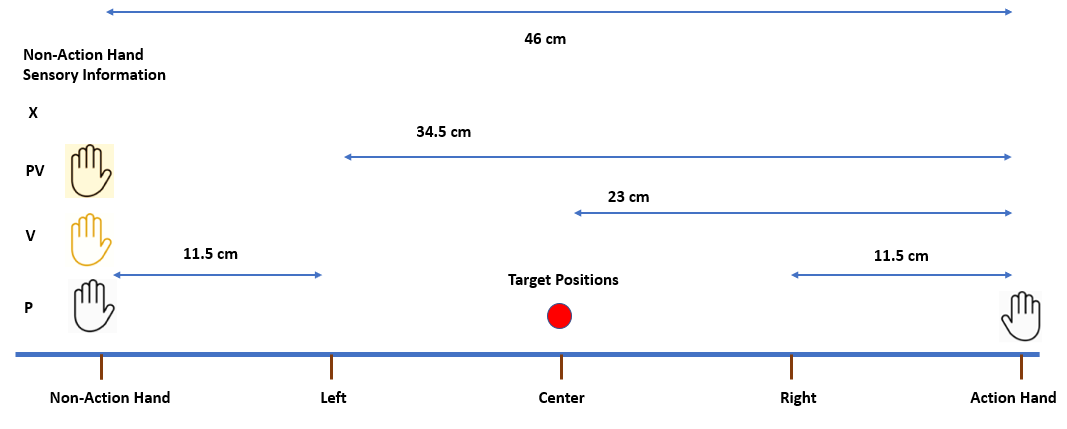
\includegraphics[width=\textwidth, keepaspectratio]{Images/exp1_task.png}
    \caption{Experimental Setup}
    \label{fig:exp1-task}
\end{figure}

\subsection{Calibration} 

At the beginning of the experiment, the participants were given oral instructions to calibrate for spatially aligning the virtual table with the physical table. Five block dots, aligned on x axis, appeared on the table with a distance of 11.5cm between them. The participant rested their right index finger on the right dock. Only the virtual hands were visible during the calibration process, whereas the physical docks were not visible in the virtual environment. Using the arrow keys on the keyboard, the participant was asked to move the rightmost black dot, such that the dot lies under their right index finger. Then, the table height was adjusted by the participant using the keypad enter and plus keys, such that the hand resting on the physical table also appeared to rest on the virtual table. The participant was then asked to rest their left index finger on the left dock, sequentially make contact with the three center dots with their right hand, and then rest the right hand on the right dock, during which the experimenter calibrated the positions of the hand at these five locations respectively.


\subsection{Procedure}


\begin{table}[t]
\centering
\resizebox{\textwidth}{!}{
\begin{tabular}{llll}
\hline 
Block & Action hand Visibility & Non-Action hand Position & Non-Action hand Visibility\tabularnewline
\hline 
Training & Visible & Lap & -\tabularnewline
Feedback & Invisible & Lap & -\tabularnewline
X & Invisible & Lap & -\tabularnewline
P & Invisible & Left dock & Invisible\tabularnewline
V & Invisible & Lap & Visible (Model hand rendered)\tabularnewline
PV & Invisible & Left dock & Visible\tabularnewline
\hline
\end{tabular}}
\caption{Experiment Block structure}
\label{table:block_structure}
\end{table}




The experiment was divided into 6 blocks. Depending upon the block, the participant was instructed regarding the placement of the left hand - either with the left index finger resting on the left dock, or the left hand resting on the participants lap. Furthermore, depending upon the block of the experiment, the left and the right hand were rendered visible or invisible.  

The participants initiated each trial by bringing their right index finger on the right dock. After an audio cue, the target is presented in one of the three target positions. On presentation of the visual target, the participant attempted to make contact with the visual target by making unspeeded reaching action with their right hand towards the target. On contact with the table, the target disappears, indicating the completion of the trial. After completion of the trial, the participant returns the right hand back to the right dock to initiate the next trial.  

The first block of the experiment was the training phase, intended to acquaint the participant with the task and the virtual environment. In the training block, the right hand was rendered visible, while the left hand was placed on the participants lap. The next block was the Feedback block, in which the right hand was rendered invisible. After the participant indicated the position of the target by making contact with the table, a green dot appeared to indicate the location where the participant had made the contact with the table. This served as feedback for the participant, to compare their responses to the actual location of the target.

In the next four blocks, the right hand was rendered invisible as a methodological constraint to introduce uncertainty in the reaching action. The presence and absence of proprioceptive and visual information of the left hand served as experimental manipulations. Proprioceptive information of the the non-action hand was manipulated by asking the participant to rest their left hand on the left dock (Proprioceptive Information present condition) or to rest their left hand on their lap (Proprioceptive Information absent Condition). The Visual information of the non-action hand was manipulated by rendering it visible (Visual Information Present Condition) or invisible (Visual Information Absent Condition). See Table \ref{table:block_structure} for a comprehensive overview of the block design.


For all participants, the first and the second block were Training and Feedback respectively. The order of the remaining four blocks was counterbalanced across participants using the Latin Square Balancing Design. The three target positions were randomized within each block. All six blocks consisted of 60 trials each, with 20 trials for each of the 3 target positions within each block. The participant thus completed a total of 360 trials across six blocks.

\subsection{Experimental Design}
\begin{table}[t]
\centering
\begin{tabular}{rlrrrrlr}
  \hline
 & Effect & DFn & DFd & F & p & p$<$.05 & pes \\ 
  \hline
1 & block & 3.00 & 60.00 & 3.482 & 0.021 & * & 0.148 \\ 
  2 & target\_pos & 1.14 & 22.89 & 10.013 & 0.003 & * & 0.334 \\ 
  3 & block:target\_pos & 3.62 & 72.38 & 1.435 & 0.235 &  & 0.067 \\ 
   \hline
\end{tabular}
\caption{Repeated measures ANOVA results with Greenhouse-Geisser Sphericity Corrections: Reach error $\sim$ Target Position * Visuo-Proprioceptive Information + (1 $\mid$ subject)}
\label{table:rm-anova}
\end{table}

The experiment was set up in a within-subject 4 x 3 factorial design, with two independent variables - Non-Action Hand Information and Target Position. Accuracy in target location estimation was operationalized as \textit{reach error}, which was computed by subtracting the actual target location from the estimated target location indicated by the participants response for each trial. Positive reach error indicates that the estimated target location was an underestimation towards the direction of the action hand, while negative reach error indicates that the estimated target location was an overestimation towards the direction of the non-action hand. Data was analyzed for the four blocks where Non-Action hand information was manipulated (X, P, V, PV). The experiment thus consisted of 12 conditions- 4 (Non-Action Hand Information conditions) x 3 (Target Position conditions). Subject-wise mean reach error was calculated for each of the 12 conditions by computing the average of mean error across trials for each condition, which served as the dependent variable.  

The Outlier criteria was determined as any participant whose any of the mean reach error values fall above Q3 + 3 x IQR or below Q1 - 3 x IQR (Q3 = Third quartile, IQR = interquartile range). On the basis of this criteria, data from one participant was excluded from the analysis.



\section{Results}

\begin{figure}
\centering       
    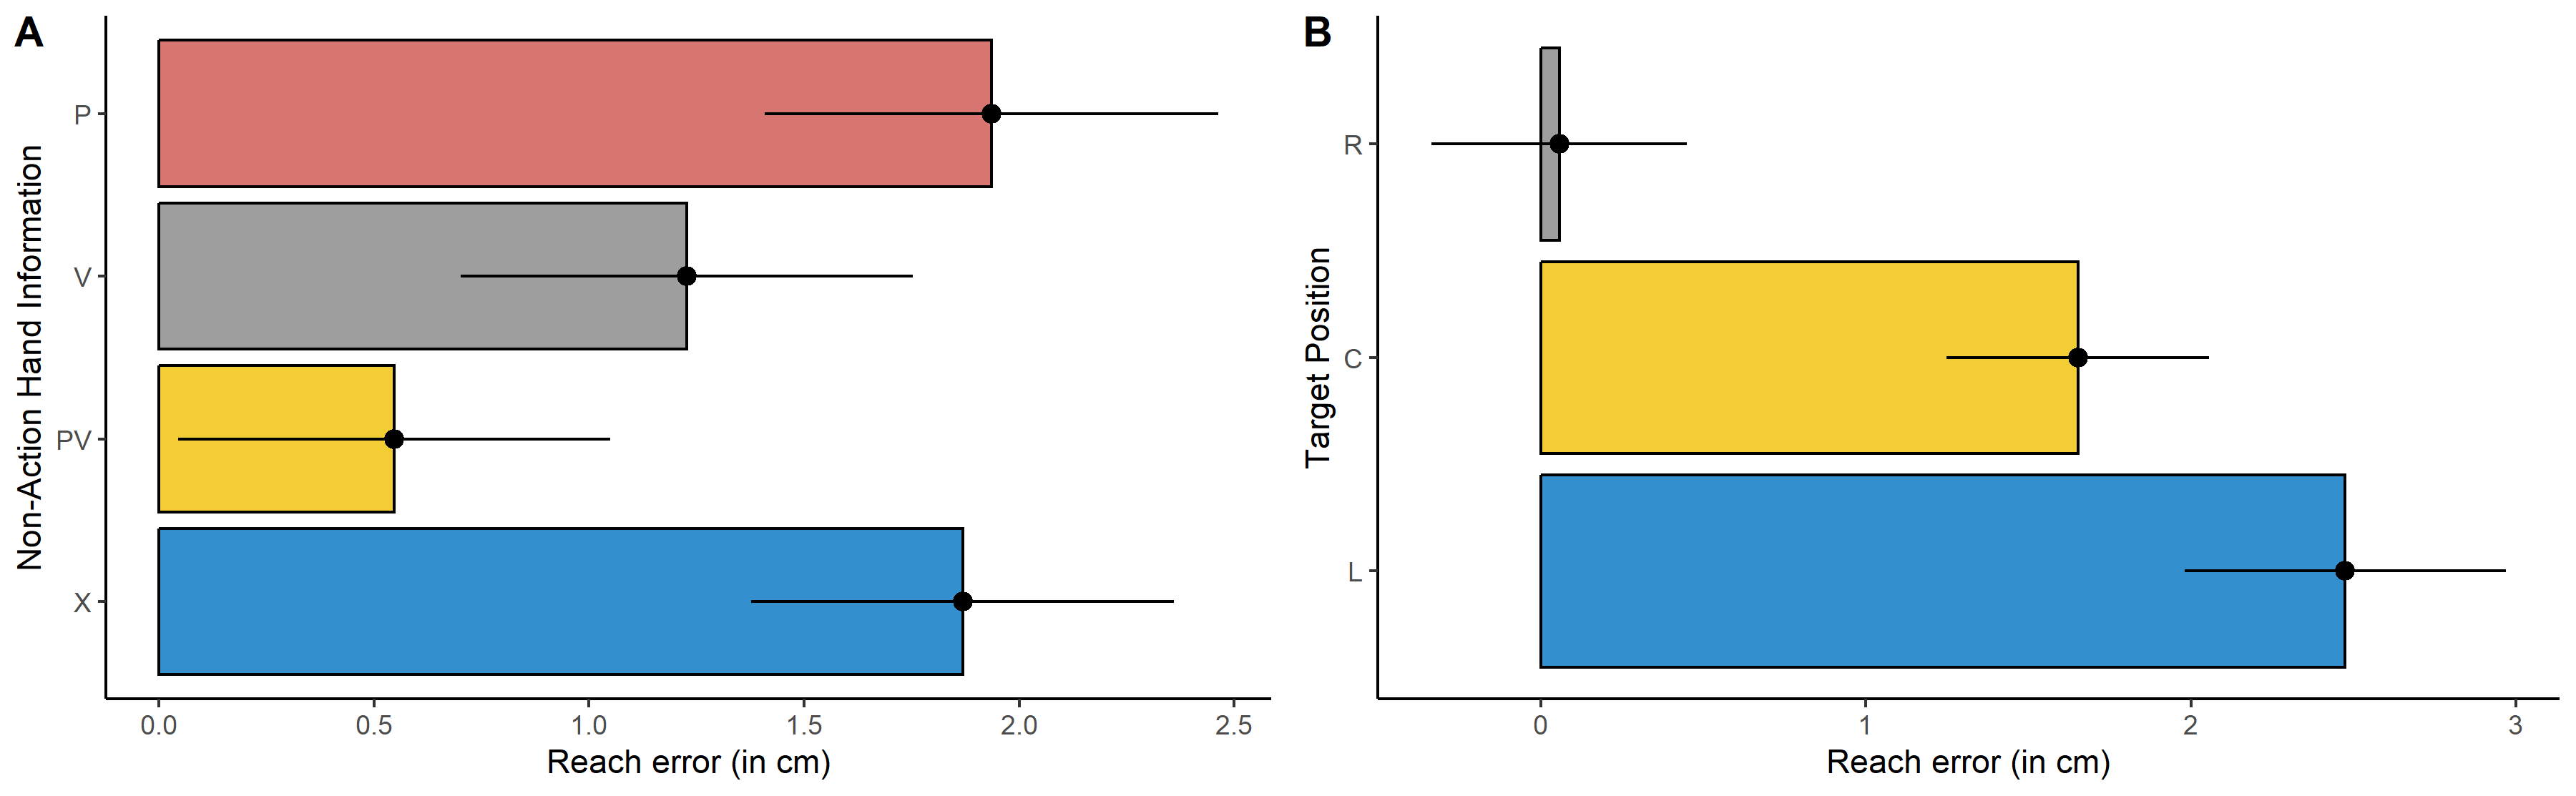
\includegraphics[width=\textwidth, keepaspectratio]{Images/exp1-mre.png}
    \caption{Effect of Non-Action hand information and Target Position on Reach error. The positive values of reach error indicate that the end point of the reach was in the direction of the action hand to the right of the target. The error bars indicate standard error of the mean.}
    \label{fig:exp1-mre}
\end{figure}


A 4 (Non-Action Hand Information: X, V, P, PV) X 3 (Target Position: Left, Center, Right) repeated measures ANOVA was performed to evaluate the effect of the two factors on magnitude of reach error. The analysis demonstrated a significant main effect of both Non-Action Hand Visibility ($F(3,60) = 3.482 , p = 0.021, \eta_{p}^{2} = 0.148$) and Target Position ($F(1.14,22.89) = 10.013, p = 0.003, \eta_{p}^{2} = 0.334$)  (See Table \ref{table:rm-anova}). No significant interaction effect between the two factors was present($F(3.62,72.38) = 1.435, p = 0.235, \eta_{p}^{2} = 0.067$). 

%Post-hoc pair-wise comparisons for analyzing the differences in the reach error between each of the four Non-Action Hand Information condition, using Bonferroni corrected paired t-test, showed that the magnitude of reach error for X and PV conditions differed significantly ($t(20) = 2.9427216, p = 0.048, d = 0.642$). Pair-wise comparisons for analyzing differences in reach error between the three target position conditions showed that reach error magnitude differed significantly between Left and Right positions ($t(20) = 3.223430, p = 0.013, d = 0.703$), and also between Center and Right positions ($t(20) = 3.728681, p = 0.004, d = 0.813$).

Post-hoc pair-wise comparisons for analyzing the differences in the reach error between each of the four Non-Action Hand Information condition, using Holm-Bonferroni corrected paired t-test, showed that the magnitude of reach error for X and PV conditions differed significantly ($t(20) = 2.9427216, p = 0.048, d = 0.642$). Pair-wise comparisons for analyzing differences in reach error between the three target position conditions showed that reach error magnitude differed significantly between Left and Right positions ($t(20) = 3.223430, p = 0.009, d = 0.703$), and also between Center and Right positions ($t(20) = 3.728681, p = 0.004, d = 0.813$).


The results of the experiment show that across all conditions, on average, there is an underestimation in the responses to the estimation of spatial location of the target, that is, the estimated target location is in the direction of the action hand relative to the actual target location. Furthermore, the subjects are more accurate (lower reach error magnitude) when both proprioceptive and visual information of the non-action hand is present (PV condition), as compared to condition in which both proprioceptive and visual information of the non-action hand is absent (X Condition). Moreover, the subjects are most accurate in the Right Target Position, lesser accurate in the Center Target Position, and least accurate in the Left Target Position. 

\section{Discussion}

%The results of this experiment suggest that subjects are more accurate in target location estimation when both visual and proprioceptive information of the hand is provided, even though the hand is reach action task irrelevant.  This result provides support to our conjecture that even task irrelevant body part in proximity to the target affects the representation of the spatial information of the target, suggesting that the target of reach action is represented in an ego-centric frame of reference with respect to the part of body near it. Furthermore, the accuracy of estimating target location is not significantly improved when just uni-sensory information of the non-action hand is present. This suggests that atleast some level of integration between visual and proprioceptive sensory signals of the hand may be necessary for the ego-centric representation of target to occur efficiently. 



The results of the experiment show that the response of the reach action is affected by the position of the target, and the sensory information of the non-action body part which is proximal to the target. The position of the target can be interpreted in two ways- as the distance to be covered by the action hand during the unfolding of action, or as the proximity to the non-action hand. Since there is no interaction effect present between the non-action hand information and the target position, the target position may be interpreted as the distance between the action hand and the target. The decrease in accuracy as the distance between the target position and initial position of action hand suggests that as the distance covered in the reach increases, the greater underestimation is observed in situations of uncertainty, which in this case is the invisibility of action hand.

Regarding the effect of non-action hand information, subjects are more accurate in target location estimation when both visual and proprioceptive information of the non-effector hand is provided, even when the body-part parameters of this hand are not seemingly relevant. This result provides support to our conjecture that even task irrelevant body part in proximity to the target affects the representation of the spatial information of the target, suggesting that the target of reach action is represented in an ego-centric frame of reference with respect to the part of body near it. Furthermore, the accuracy of estimating target location is not significantly improved when just uni-sensory information of the non-action hand is present. This suggests that atleast some level of integration between visual and proprioceptive sensory signals of the hand may be necessary for the ego-centric representation of target to occur efficiently.

However, if the spatial encoding of the the target is indeed anchored to the sensory information which specifies the position of the body-part proximal to the target, the expectation is that the proximity to the target should increase the accuracy of the spatial representation of the target. However, the results indicate the opposite. Thus overall, this suggests that there are two processes which additively influence the spatial encoding of the target- i) underestimation when the reaches are over longer distances, and ii) biasing the target position towards the non-action hand (thus increasing the accuracy) when the target's spatial information is anchored to it when its multi-sensory information is present.



%What exactly does ego-centric anchoring achieve? One possibility is that the anchoring causes a reduced uncertainty regarding the target position, which is indicated by main effect of condition with more accurate action when both proprioceptive and visual information regarding non-target hand was present. However, the lack of increase in accuracy when the target is closer to the non-action hand suggests that there is an interaction between the two processes of i) underestimation when the reaches are over longer distances, and ii) Biasing the target position towards non-action hand when the target representation is anchored to it.







%\chapter{Model}
\label{model}
\lhead{Chapter 2. \emph{Model}} 

\section{Introduction}
One of the ways to understand perception, is that perception is an inferential process, in which the agent attempts to infer the most probable state of the world, by using the sensory inputs and previous knowledge that it possesses regarding the state of the world. 

Thus, in the case of reaching action, one of the computational problems that the agent's cognitive system needs to solve is to infer the location of the target, when raw sensory inputs (here, visual) about the target are provided.  

This computation can be modelled using a simple Bayesian approach. For every possible target location, the system assigns a probability regarding how likely that particular target location is. The estimated target location is the location with the highest probability. 
The allocation of probabilities to different target locations is done in two parts.

\begin{enumerate}

\item Probabilities are assigned on basis of the raw sensory input of the target. If the actual location of the target is $s$, highest probability will be assigned to the location $s$. However, since there is noise inherently present in the system, probabilities are assigned to other locations as well. Mathematically, this probability distribution function may follow a normal distribution which is centered (mean) at $s$, and with variance $ \sigma_m^2$ , which represents the noise or the measurement error in the system. Therefore,

$ P(x|s) = N(x; s, \sigma_m^2) $, where x is the observation, and s is the actual location of the target. 

\item Probabilities are assigned on basis of the prior knowledge which the agent possesses regarding how likely each target locations are. This probability distribution does not take into account the actual location of the target, but merely represents the prior beliefs that the agent possess about how likely each target location is. If each location is equally likely, $ P(s) = U(a,b)$ , where a and b are the bounds to the target location space.

\end{enumerate}

The process of inference involves combining the information from observation (likelihood distribution) and expectation (prior distribution). This posterior probability distribution represents the systems beliefs for the probability of each possible location for the target.   


\section{The Bayesian Model}

We claim that, in situations of uncertainty, the body schema acts as a prior and influences the belief that certain target locations are more likely than the others. We are modelling these prior beliefs as a normal distribution function, with parameters, $\mu_p$ and $\sigma_p^2$. $\mu_p$ represents which target location is believed to be most likely. $\sigma_p^2$ denotes the confidence the agent has in the prior. Higher value of  $\sigma_p^2$ , that is a flatter prior distribution indicates that the prior is not very informative, and the sensory observation (likelihood distribution) will be more informative. The intuition behind this is that, the prior biases the posterior away from the sensory measurement, but the magnitude of this "pull" would depend upon how sharp or flat the prior distribution is. 



Prior distribution : $ P(s_{hyp}) = N(s_{hyp};  \mu_p,  \sigma_p^2) $ \\
Likelihood function : $ P(x|s_{hyp}) = N(x;  s_{hyp},  \sigma_m^2) $ \\
Posterior distribution : $ P(s_{hyp} | x) = N ( s_{hyp};  \frac{J_p \mu_p + J_m x}{J_p + J_m} ,  \frac{1}{J_p + J_m}$ ) 

where, \\
$ J_p = \frac{1}{\sigma_p^2}$ \\
$ J_m = \frac{1}{\sigma_m^2}$ \\
$x$ = Noisy sensory observation \\
$s_{hyp}$ = Hypothesized location of the target \\


Ultimately, the estimated target location is equivalent to the mean of the posterior distribution, that is, the value of $s_{hyp}$ which has the highest probability assigned to it. Thus, the estimated target location is given by,
$\hat{s} = \frac{J_p \mu_p + J_m x}{J_p + J_m} $ 
This is the response that the agent indicates in the target location estimation task.

\subsection{Response distribution}

Assume that the actual location of the stimuli is $s$. For a given $s$, the noisy sensory measurement of the target $x$ is not a constant, but a random variable. Therefore, on repeated presentation of the target at a particular location $s$, the estimated target location $\hat{s}$ will be a random variable, with an associated probability distribution.

Using properties of linear combination of random variables, this distribution is given by,

\begin{equation} \label{eq:rd}
     P(\hat{s} | s) = N (\hat{s};  \frac{J_p \mu_p + J_m s}{J_p + J_m} , \frac{J_m}{(J_p + J_m)^2} ) 
\end{equation}



\section{Claim}

We claim that when the action hand is invisible, the beliefs will be biased for target locations near the action hand, that is, the prior mean will be nearer to the action hand. This may explain the behavioural results of displacement of estimated target locations towards the action hand. Furthermore, we hypothesize that the the different non-action hand conditions will affect the prior variance. X condition should exhibit least prior variance and PV condition should exhibit higher prior variance. Since prior variance denotes the confidence that the subject has in the prior information, we claim that the visuo-proprioceptive information of the non-action hand reduces the bias induced by the uncertainty due to the non-visible non-action hand by decreasing the confidence in this bias.


To summarize,

\begin{enumerate}
    \item When action hand is visible, no uncertainty, no bias towards the action hand.
    \item When action hand is invisible, higher uncertainty, therefore estimated target locations are biased towards the action-hand. $\mu_p$ will be near to the action hand
    \item When non-action hand visuo-proprioceptive information is available, the confidence in the bias induced by the non-visible action hand is reduced (high $\sigma_p$ ). Thus, the agents are more accurate in estimating the target location in PV condition.
\end{enumerate}


\section{Model fitting}

We fit the response distribution model given in Equation \ref{eq:rd} to the behavioural data. For each participant, and for each block condition, we estimated the two parameters $\mu_p$ and $\sigma_p$. The values of $\sigma_m$ were determined experimentally by calculating the standard deviation of the estimated target location in the Practice block, when the action hand was visible. The reasoning behind this is that, when action hand is visible, there is no bias induced due to uncertainty which reflects in the information captured in the prior distribution. Thus, the variability is the responses should mirror the variability in the measurement distribution (that is, the likelihood distribution).

\section{Further steps}

\begin{enumerate}
    \item Simulate how model behaves for different values of parameters. Check if my model can capture my hypothesis. DONE. I have inputted various values of the parameters into the model and simulated the response distribution. The model behaviour is consistent with my hypothesis.
    
    \item Recover parameters for different values of parameters. DONE! Parameter recovery is happening. 
    
    \item Fit the model to the data. DONE. I have got some estimates of the parameters. For estimating the parameters, I have set the bounds of sig.p as [0.001, Inf) and mu.p as [0, -46]. 
    
    \item Is my model a good fit to the data? Stuck here. How do I figure this out?
    
    \item While identifying outliers in the estimated sig.p values, 5 extreme outliers were identified.
    
    
\end{enumerate}

%\chapter{Experiment 2}
\label{exp2.0}
\lhead{Chapter 4. \emph{Experiment 2}} 

\section{Introduction}

In the previous chapter, we found evidence that the spatial encoding of the reach action target is influenced by the multi-modal nature of sensory information about the body-part in proximity to the target, with increased accuracy when the nature of this information is multi-modal, as compared to uni-sensory information. What does the multi-modal sensory information regarding the body imply? According to \citeauthor{ataria2021body}, signals from multiple sources like vision and proprioception are integrated to construct a representation of the body (\textit{body schema}, which specifies certain parameters like the position of the body part. Thus, one of the functions of multi-sensory integration is to compute reliable estimates of the location of the body part, by integrating the estimates provided by uni-sensory cues on the basis of its reliability and the relevance attributed to the particular modality \citep{limanowski2016integration, noel2018peri, kording2007causal, van1999integration}. Thus, it seems that this mechanism of multi-sensory integration which specifies the position of the body-part may underlie the spatial encoding of the target of reach action which is located in its proximity.

Generally, vision and proprioception provide congruent estimates about the position of the body. However, inducing discrepancy between the estimates provided by vision and proprioception allow us to probe further into proximal body-part multi-sensory integration mechanism underlying the spatial encoding of target. Therefore, in the following experiment, we manipulated the spatially discrepancy between the actual position of the non-action target proximal hand and its visual input, by spatially displacing the visually rendered hand in an Immersive Virtual Reality environment. The objective of this experiment was to understand how the target location estimation in reach action is affected by the spatial discrepancy between the estimate provided by proprioception and vision about the proximal body-part location. Specifically, we aimed to test the hypothesis that congruency between visual and proprioceptive estimates of proximal body-part location will lead to more accurate encoding of the spatial information of the target. We also aimed to understand how the differences in proximity to the body-part with incongruent estimates from visuo-proprioceptive inputs affects the target location estimation. 


%What is the location of my hand? The answer to this question is provided by inputs from multiple sensory modalities like vision and proprioception. Visual and proprioceptive information is integrated to infer an estimate regarding the location of the hand ~\citep{van1999integration}. Generally, vision and proprioception provide congruent estimates about the location of the body. However, inducing discrepancy between the estimates provided by vision and proprioception through experimental manipulation allows us to understand how the integration between the two modalities affects the representation of the target of the reach action.

%In the following experiment, we manipulated spatial discrepancy between the actual position of the hand and the visual input of the task-irrelevant hand, by spatially displacing the visually rendered hand in an Immersive Virtual Reality environment. The objective of this experiment was to understand how the target location estimation is affected by the spatial discrepancy induced between the estimate provided by proprioception and vision of the hand. We expected that reach error will be lowest in the condition where vision and proprioception are congruent. However, for visuo-proprioceptive incongruent conditions, we hypothesized that the way visuo-proprioceptive discrepancy affects the reach error is dependent upon the distance between the target and the non-action hand. 

\section{Method}

\subsection{Participants}
Nineteen right-handed subjects(2 Females, Mean age = 22.68, Range = 18-33) were recruited to participate in the experiment. All participants reported normal or corrected to normal vision. They were naive to the purpose of the experiment and the experimental procedure, and had provided written consent to participate in the study according to the norms approved by the Institute Ethics Committee (IEC) of Indian Institute of Technology, Kanpur. 

\subsection{Materials and Apparatus}
The participants sat across a table with surface area dimensions of 120cm x 50cm. Two coin-shaped docks (2.5 cm diameter) were attached to the table with a distance of 46 cm between them at the center of the table. A cylindrical barrier of 2.5cm height was attached around the right dock. The participant sat with their arms resting comfortably on the table, with the right and left docks serving as resting positions for the right and left index fingers respectively. Hand motion and position was tracked with Ultraleap Leap Motion Controller. The virtual reality environment was displayed on Oculus Rift S Head-mounted Display, and developed using Unity Game Engine. The virtual scene consisted of a virtual table situated in a black room. The virtual table was spatially aligned to the physical table at which the participant sat. The target of the reach was a red dot of 0.5cm in diameter. 

\subsection{Procedure}

The experiment began with a calibration session, similar to the session performed in Experiment 1 (Refer Chapter \ref{exp1}). The experiment consisted of 5 Experimental blocks which were interleaved with filler blocks. For the experimental blocks, the participants were instructed to place their left hand on the dock, whereas for the filler blocks, the left hand was placed on the lap. The experimental blocks differed in the position at which the left hand was rendered visually in the virtual scene. The visual rendering of the left hand, henceforth termed as the visual hand, was positioned at five locations - congruent to the left hand placed at the left dock (henceforth termed as the proprioceptive hand), 5.75cm, and 11.50cm to the right of proprioceptive hand, and 5.75cm and 11.50cm to the left of the proprioceptive hand. The order of the experimental blocks was counterbalanced across participants using Latin Square counterbalancing design. 

\begin{figure}
\centering       
    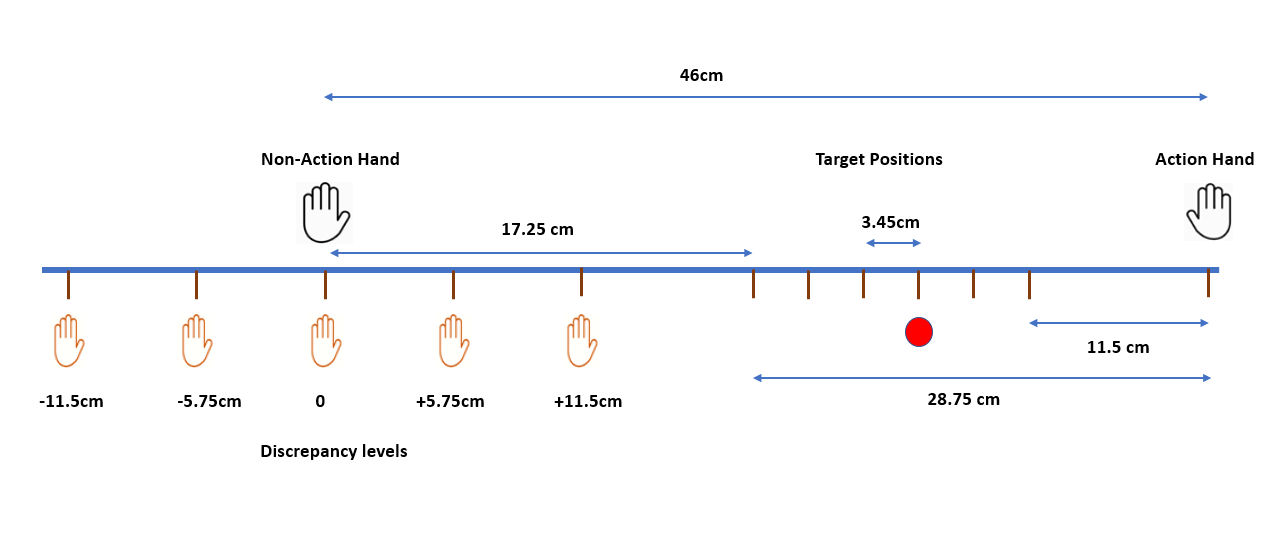
\includegraphics[width=\textwidth, keepaspectratio]{Images/exp2_task.png}
    \caption{Experimental Setup}
    \label{fig:exp2-task}
\end{figure}

Within each block, the target appeared at one of the following 6 locations along the axis joining the two docks, at a distance of  28.75, 25.30, 21.85, 18.40, 14.95, and 11.50 cm from the action hand (see Figure \ref{fig:exp2-task}). The experimental blocks each consisted of 10 x 6 (target positions) = 60 trials, while the filler blocks consisted of 5 trials each. 

The task performed by the participant was same as that of experiment 1. Each trial was initiated by bringing the right index finger on the right dock. On an audio cue, the target appeared at one of the above mentioned target locations, after which the participant attempted to make contact with the target with their right index position. The trial ended with the disappearance of the target after the contact was detected between the table and the right index finger. The participant brought the right hand back to the right dock to initiate the next trial. Throughout the course of the experiment, the right (action hand) was rendered invisible. 

\begin{table}[t]
\centering
\resizebox{\textwidth}{!}{
\begin{tabular}{llrr}
  \hline
  Model & Fixed effect & AIC & BIC \\
  \hline
  Null Model & None &	28746 &	28779 \\
  Discrepancy Model & Discrepancy	& 28731	& 28770 \\
  AHT Model & AHT &	28698 &	28737 \\
  Additive Model & Discrepancy + AHT	& 28683	& 28729 \\
  \textbf{Interaction Model} & \textbf{Discrepancy + AHT + (Discrepancy * AHT)} & \textbf{28666} & \textbf{28719}\\
   \hline
\end{tabular}}
\caption{AIC and BIC Values for fitted Linear Mixed Effect models. Random effects of all models consisted of intercepts for subjects and by-subject random slopes for effect of discrepancy ( $1 + discrepancy | subject$ ). The interaction model has the lowest AIC and BIC value. }
\label{table:lme-models}
\end{table}

  
 

\subsection{Experimental Design}

The accuracy of the spatial encoding of the target in reach action was operationalized as \textit{reach error}, which was computed as the difference between the actual location of the target and the estimated location of the target, indicated by the participant by the end-point of the reach action. Positive reach error indicates that the relative to the actual position of the target, the estimate of the target location is in the direction towards the action hand. On the other hand, negative reach error indicates that target location estimate is to the left of the actual target location in the direction of the the non-action hand. 

The experiment was set-up in a within-subjects experimental design, with reach error as the dependent variable. The two independent variables that were experimentally manipulated were - i) The non-action hand visuo-proprioceptive spatial discrepancy, that is, the distance between the actual position of the hand (proprioceptive hand) and the visual rendering of the hand (visual hand), and ii) The distance between the proprioceptive hand and target (PHT). 

\section{Results}
\begin{figure}[t]
\centering       
    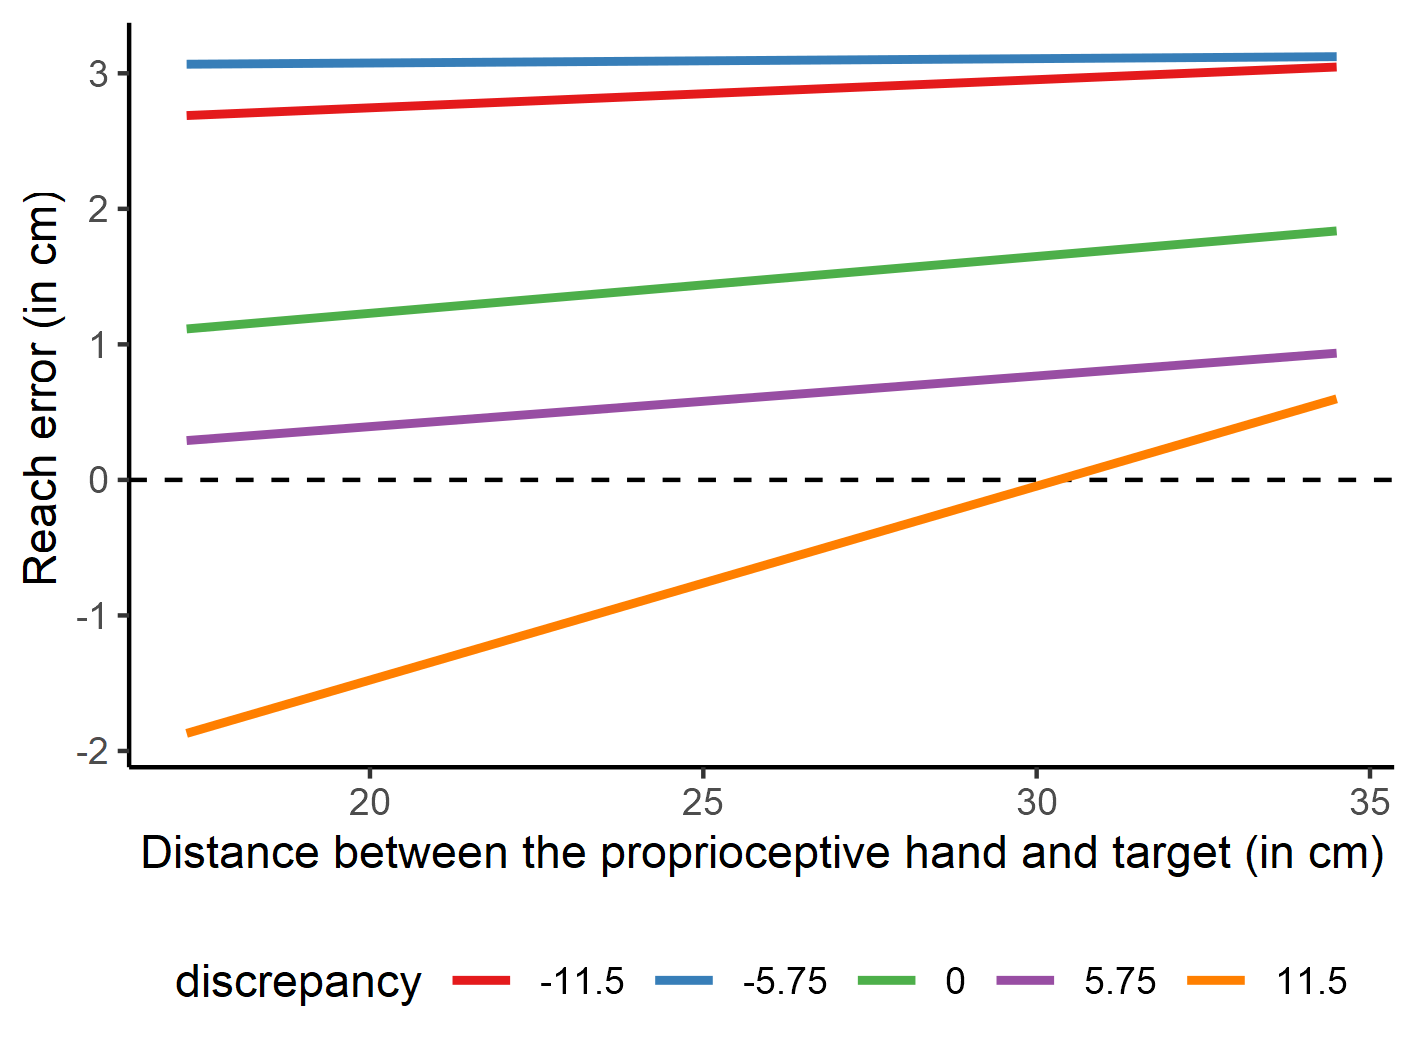
\includegraphics[scale=0.8]{Images/exp2_results.png}
    \caption{Reach error as a function of spatial discrepancy between the position of visual hand and the position of actual (proprioceptive) non-action hand. Each panel shows the distance between the target and the initial position of the action hand (AHT). Negative reach error indicates that the estimation of the target location was in the direction of the non-action hand towards the left, while positive reach error indicates that the location of the target was estimated in the direction of action hand towards the right of the actual location of the target.}
    \label{fig:exp2_re-pht}
\end{figure}

%\subsection{Data Analysis}

To understand the effect of visuo-proprioceptive spatial discrepancy and the distance from the target from the proprioceptive hand (PHT) on the reach error, we performed a linear mixed effects analysis using the \emph{lme4} ~\citep{bates2014fitting} and \emph{lmerTest} packages in R. Random effects of all models that we fit consisted of intercepts for the subjects and by-subject random slopes for the effect of discrepancy. Table \ref{table:lme-models} reports the AIC and BIC values of the models that we fit. Furthermore, we performed Likelihood Ratio Test to compare the models and as a criteria for model selection. Refer Appendix \ref{App-exp2-analysis} for the results of the Likelihood Ratio test. 

The AIC, BIC, and the results of the Likelihood Ratio Test reveal that the best fit model consisted of discrepancy and PHT as the fixed effects, along with an interaction between the two predictors. There were no obvious deviations from homoscedasticity and normality on the basis of visual inspection of residual plots. Furthermore, we checked for multi-collinearity between the predictors by using Variance Inflation Factor (VIF) as a measure of collinearity using the package \emph{performance} in R. The results show low correlation (VIF < 2) between the fixed effect terms of the best-fit model (see Table \ref{table:collinearity}).

Moreover, we performed bootstrapping to get credible confidence intervals at 95\% for the estimates of the fixed effects (see Table \ref{Table:Bootstrapped estimates}). None of the confidence intervals for the fixed effects contain the value 0, which further supports the significance of the effects of the three predictors (discrepancy, PHT, and interaction) on the reach error. 


\section{Discussion}
The results of the Linear Mixed Effects analysis shows that the interaction between the spatial discrepancy between the visual and proprioceptive inputs of the non-action hand and the distance between the target and the actual hand has a statistically significant effect on reach error. This suggests that the way visuo-proprioceptive spatial discrepancy of proximal non-action hand affects the target estimation depends upon the distance of the target from the the non-action hand. Figure \ref{fig:exp2_re-pht} shows the effect of proprioceptive hand and target distance (PHT) on reach error at different levels of discrepancy.

When the visual and the proprioceptive information provide congruent estimates for the location of the non-action hand (discrepancy = 0), the target location is underestimated towards the action hand. Reach accuracy is improved as the proximity between the target and the proprioceptive hand increases. As the visuo-proprioceptive discrepancy increases, with the visual hand being rendered closer to the target (discrepancy = +5.75cm), the reaches are more accurate. This suggests that the visual hand may be used as an anchor for the target representation due to its proximity to the target despite the discrepancy between the visual and proprioceptive inputs of the hand. However, as the discrepancy increases further, with visual hand moving even closer to the target (discrepancy = 11.5cm), the estimate of the target location is pulled towards the visual hand, as indicated by the negative values of the reach errors. This "pull" effect diminishes as the distance between the target and the proprioceptive hand increases. However, the close proximity of visual hand and target seems to increase the accuracy even though the visuo-proprioceptive discrepancy is high and when the target is far from the proprioceptive hand. In contrast, when the visuo-proprioceptive discrepancy is induced by rendering the visual hand away from the targets (discrepancy = -5.75cm and -11.50cm), overall high values of reach error are observed. The proximity between the proprioceptive hand and target do not have an effect on the reach error, in this case.

Overall, these results suggest that it is not merely the spatial discrepancy between the visual and proprioceptive information that affects the accuracy in target location estimation. Rather, the proximity of the visual hand to the target biases the estimation of the target in its direction, suggesting that the spatial encoding of the target may be anchored to the visual information of the body part in proximity.  

%These results contradict the hypothesis that of multi-sensory model to understand how target may be represented with respect to it. The model was that unisensory estimates will be combined to get a more reliable estimate. that means, the reliability will be more for the less discrepancy conditions and less for higher discrepancy conditions. There are thus two aspects, how reliable it is, and how close it is to the target. At negative discrepancy, 


 
\section{Bayesian Causal Inference Model}

To further interpret the results of the experiment, we qualitatively inspected the predictions of Bayesian Causal Inference Model and interpreted our results with respect to it. We find that there is no effect of distance from hand position predicted by the BCI model. On the other hand, the distance from the visual hand has a significant effect. 





































\chapter{Visuo-proprioceptive spatial discrepancies in proximal body-part}
\label{exp2}
\lhead{Chapter 4. \emph{Visuo-proprioceptive spatial discrepancies in proximal body-part}} 

\section{Introduction}

In the previous chapter, we discussed evidence supporting the hypothesis that multi-sensory visuo-proprioceptive integration mechanisms of proximal body-part plays a role in reach target's spatial encoding. But how exactly is the multi-sensory integration involved in the target's spatial encoding? Let us consider two hypothesis which may plausibly explain the implication of the integration mechanism in reach target's spatial encoding.

%The experiment described in Chapter \ref{exp1} suggests that multi-sensory visuo-proprioceptive integration mechanisms of proximal non-effector body-part play a role in encoding of the spatial information of the reach target. To understand how multi-sensory integration mechanism plays a role in spatial encoding of the reach target, let us consider two hypothesis regarding the integration mechanism.

\begin{figure}[t]
\centering       
    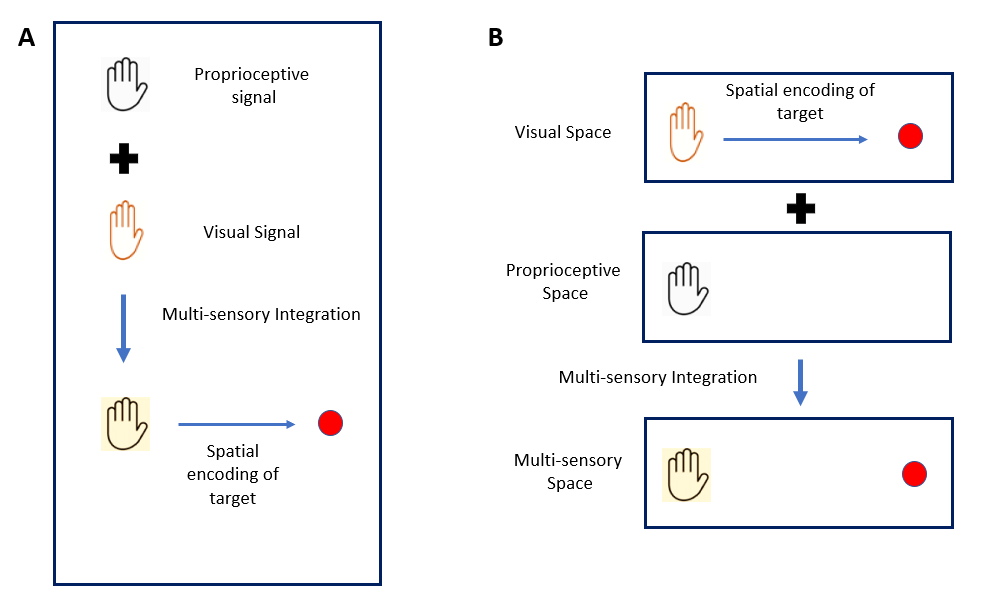
\includegraphics[width=\textwidth, keepaspectratio]{Images/ms_mechanisms.png}
    \caption{Two hypothesis regarding spatial encoding of the reach target. In A), the filled hand denotes the hand position inferred from the multi-sensory integration of visual and proprioceptive uni-sensory signals. The target's spatial location is encoded relative to this inferred hand position. In B) The target's spatial location is encoded relative to the visual signal in the visual space. The visual space is then integrated with the proprioceptive space to construct a multi-sensory representation of body-schema and surrounding peri-personal space.}
    \label{fig:ms-mechanisms}
\end{figure}

\subsection{Spatial encoding with respect to the inferred position of proximal body-part}

One of the mechanisms postulated regarding the specification of body's spatial information in the representation of body (that is, the body schema) is that of visuo-proprioceptive multi-sensory integration. Here, the functional role of multi-sensory integration is to compute reliable estimates of the location of the body part, by integrating the estimates provided by uni-sensory cues on the basis of its reliability and the relevance attributed to the particular modality \cite{limanowski2016integration, noel2018peri, kording2007causal, van1999integration}. In this light, the way multi-sensory integration could be involved in spatial encoding of the reach target is as follows- multi-sensory integration results in the inference of a reliable estimate of proximal body-part's spatial location, and thereafter, the spatial location of the reach target is represented with respect to this inferred spatial location. A schematic of this conjecture is shown in Figure \ref{fig:ms-mechanisms} (A).


\subsection{Spatial encoding with respect to the visual signal of proximal body-part}
An alternative hypothesis is that the spatial encoding of the target could occur with respect to the estimate of the body-part position provided by its visual signal. This visual space, containing a map of visual objects- body part and the target, is then integrated with the proprioceptive space containing a map of proprioceptive objects (see Figure \ref{fig:ms-mechanisms} (B)). The plausibility of this hypothesis is supported by several empirical studies. For instance, the reach target is a visual object, and several studies have shown increases in accuracy of reaching, when visual "landmarks" are in proximity to the reach target \cite<eg.>{conti1980role}, suggesting the occurrence of allocentric encoding of reach target. Furthermore, several studies have also suggested that spatial encoding in allocentric reference frames is used in combination with egocentric representation \cite{byrne2010interactions, schutz2013gaze}, although the literature here refers to eye-centered egocentric representation. Nevertheless, it is plausible that the spatial encoding of visual target is with respect to the visual information, and this visual space is then integrated with proprioceptive space, to construct a multi-sensory representation of space which is characteristic of peri-personal space representation. 


\section{Experiment 2}

To test for these competing hypothesis, we conducted an experiment in which we manipulated the spatial discrepancy between the actual position of the non-action target proximal hand and its visual input, by spatially displacing the visually rendered hand in an Immersive Virtual Reality environment. The objective of this experiment was to understand how reach target location estimation was affected by the spatial discrepancy in the estimates provided by visual and proprioceptive inputs of the body-part (non-action hand) proximal to the target. We also aimed to qualitatively compare which of the mechanistic hypotheses described above explains the the reach accuracy results. If the inferred position of the proximal hand systematically affects the target location estimation, it would suggest that Hypothesis 1 may be the multi-sensory mechanism that could underlie body-proximal reach target spatial encoding. On the other hand, if the proximity to the visual hand systematically affects the target location estimation, Hypothesis 2 may be the mechanism underlying the reach target spatial encoding.


\subsection{Method}

\subsubsection{Participants}
Nineteen right-handed subjects(2 Females, Mean age = 22.68, Range = 18-33) were recruited to participate in the experiment. All participants reported normal or corrected to normal vision. They were naive to the purpose of the experiment and the experimental procedure, and had provided written consent to participate in the study according to the norms approved by the Institute Ethics Committee (IEC) of Indian Institute of Technology, Kanpur. 

\subsubsection{Materials and Apparatus}
The participants sat across a table with surface area dimensions of 120cm x 50cm. Two coin-shaped docks (2.5 cm diameter) were attached to the table with a distance of 46 cm between them at the center of the table. A cylindrical barrier of 2.5cm height was attached around the right dock. The participant sat with their arms resting comfortably on the table, with the right and left docks serving as resting positions for the right and left index fingers respectively. Hand motion and position was tracked with Ultraleap Leap Motion Controller. The virtual reality environment was displayed on Oculus Rift S Head-mounted Display, and developed using Unity Game Engine. The virtual scene consisted of a virtual table situated in a black room. The virtual table was spatially aligned to the physical table at which the participant sat. The target of the reach was a red dot of 0.5cm in diameter. 

\subsubsection{Procedure}

The experiment began with a calibration session, similar to the session performed in Experiment 1 (Refer Chapter \ref{exp1}). The experiment consisted of 5 Experimental blocks which were interleaved with filler blocks. For the experimental blocks, the participants were instructed to place their left hand on the dock, whereas for the filler blocks, the left hand was placed on the lap. The experimental blocks differed in the position at which the left hand was rendered visually in the virtual scene. The visual rendering of the left hand, henceforth termed as the visual hand, was positioned at five locations - congruent to the left hand placed at the left dock (henceforth termed as the proprioceptive hand), 5.75cm, and 11.50cm to the right of proprioceptive hand, and 5.75cm and 11.50cm to the left of the proprioceptive hand. The order of the experimental blocks was counterbalanced across participants using Latin Square counterbalancing design. 

\begin{figure}
\centering       
    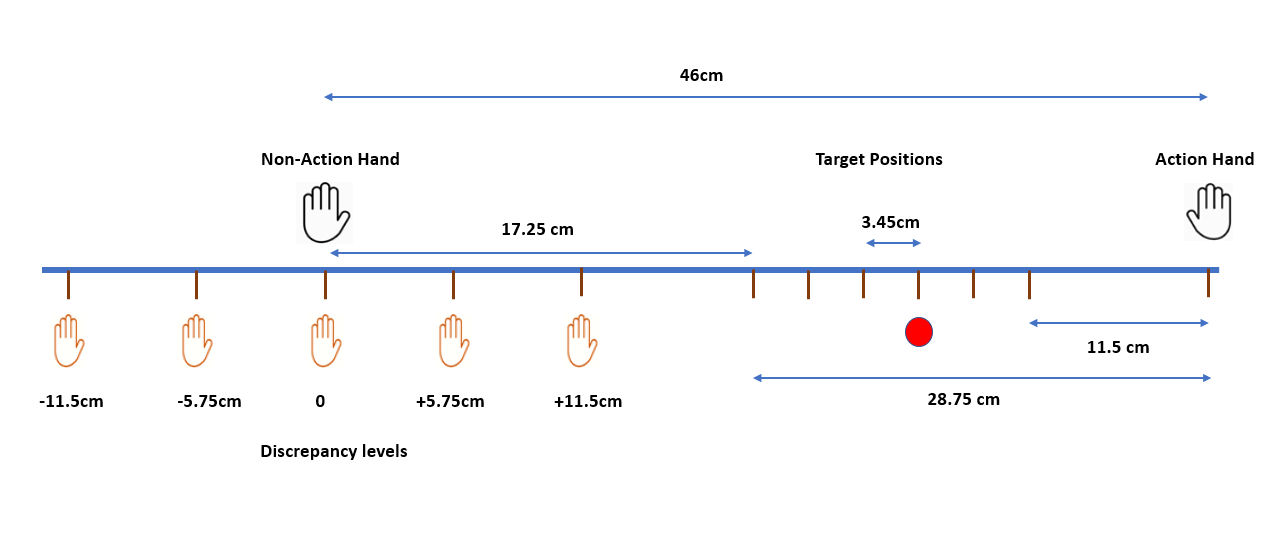
\includegraphics[width=\textwidth, keepaspectratio]{Images/exp2_task.png}
    \caption{Experimental Setup}
    \label{fig:exp2-task}
\end{figure}

Within each block, the target appeared at one of the following 6 locations along the axis joining the two docks, at a distance of  28.75, 25.30, 21.85, 18.40, 14.95, and 11.50 cm from the action hand (see Figure \ref{fig:exp2-task}). The experimental blocks each consisted of 10 x 6 (target positions) = 60 trials, while the filler blocks consisted of 5 trials each. 

The task performed by the participant was same as that of experiment 1. Each trial was initiated by bringing the right index finger on the right dock. On an audio cue, the target appeared at one of the above mentioned target locations, after which the participant attempted to make contact with the target with their right index position. The trial ended with the disappearance of the target after the contact was detected between the table and the right index finger. The participant brought the right hand back to the right dock to initiate the next trial. Throughout the course of the experiment, the right (action hand) was rendered invisible. 


\subsubsection{Experimental Design}

The accuracy of the spatial encoding of the target in reach action was operationalized as \textit{reach error}, which was computed as the difference between the actual location of the target and the estimated location of the target, indicated by the participant by the end-point of the reach action. Positive reach error indicates that the relative to the actual position of the target, the estimate of the target location is in the direction towards the action hand. On the other hand, negative reach error indicates that target location estimate is to the left of the actual target location in the direction of the the non-action hand. 

The experiment was set-up in a within-subjects experimental design, with reach error as the dependent variable. The two independent variables that were experimentally manipulated were - i) The non-action hand visuo-proprioceptive spatial discrepancy, that is, the distance between the actual position of the hand (proprioceptive hand) and the visual rendering of the hand (visual hand), and ii) The distance between the initial position of the action hand and target (AHT). 

\subsection{Data Analysis}

\begin{table}[t]
\centering
\resizebox{\textwidth}{!}{
\begin{tabular}{llrr}
  \hline
  Model & Fixed effect & AIC & BIC \\
  \hline
  Null Model & None &	28746 &	28779 \\
  Discrepancy Model & Discrepancy	& 28731	& 28770 \\
  AHT Model & AHT &	28698 &	28737 \\
  Additive Model & Discrepancy + AHT	& 28683	& 28729 \\
  \textbf{Interaction Model} & \textbf{Discrepancy + AHT + (Discrepancy * AHT)} & \textbf{28666} & \textbf{28719}\\
   \hline
\end{tabular}}
\caption{AIC and BIC Values for fitted Linear Mixed Effect models. Random effects of all models consisted of intercepts for subjects and by-subject random slopes for effect of discrepancy ( $1 + discrepancy | subject$ ). The interaction model has the lowest AIC and BIC value. }
\label{table:lme-models}
\end{table}

  
 


To understand the effect of visuo-proprioceptive spatial discrepancy on the reach error, we performed a linear mixed effects analysis using the \emph{lme4} ~\cite{bates2014fitting} and \emph{lmerTest} packages in R. We considered visuo- proprioceptive spatial discrepancy and the distance from action hand (AHT) as fixed effects in our models. Random effects of all models that we fit consisted of intercepts for the subjects and by-subject random slopes for the effect of discrepancy. Table \ref{table:lme-models} states the fixed effects of the various fitted models and their Akaike information criterion (AIC) and Bayesian Information Criteria (BIC) values. Likelihood Ratio Test was performed to compare the models and as a criteria for model selection. Refer Appendix \ref{App-exp2-analysis} for the results of the Likelihood Ratio test. 

The AIC, BIC, and the results of the Likelihood Ratio Test reveal that the best fit model consisted of discrepancy and AHT as the fixed effects, along with an interaction between the two predictors (see Table \ref{table:lme-bestfit-fixedeffect}). There were no obvious deviations from homoscedasticity and normality on the basis of visual inspection of residual plots (See Figure \ref{fig:lme-residual} and Figure \ref{fig:lme-norm}). Furthermore, we checked for multi-collinearity between the predictors by using Variance Inflation Factor (VIF) as a measure of collinearity using the package \emph{performance} in R. The results show low correlation (VIF < 2) between the fixed effect terms of the best-fit model (see Table \ref{table:collinearity}).

Moreover, we performed bootstrapping to get credible confidence intervals at 95\% for the estimates of the fixed effects (see Table \ref{Table:Bootstrapped estimates}). None of the confidence intervals for the fixed effects contain the value 0, which further supports the significance of the effects of the three predictors (discrepancy, AHT, and interaction) on the reach error. 

Thus, the results of the Linear Mixed Effects analysis shows that the interaction between the spatial discrepancy between the visual and proprioceptive inputs of the proximal non-action hand and the distance between the target and the action hand has a statistically significant effect on reach error. This suggests that the way visuo-proprioceptive spatial discrepancy of proximal non-action hand affects the target estimation depends upon the distance of the target from the the action hand. Therefore, to interpret the results, we will consider the effect of visuo-proprioceptive discrepancy separately at different distances of target from the action hand. 



\subsection{Support for visual anchoring mechanism}
\begin{figure}[t]
\centering       
    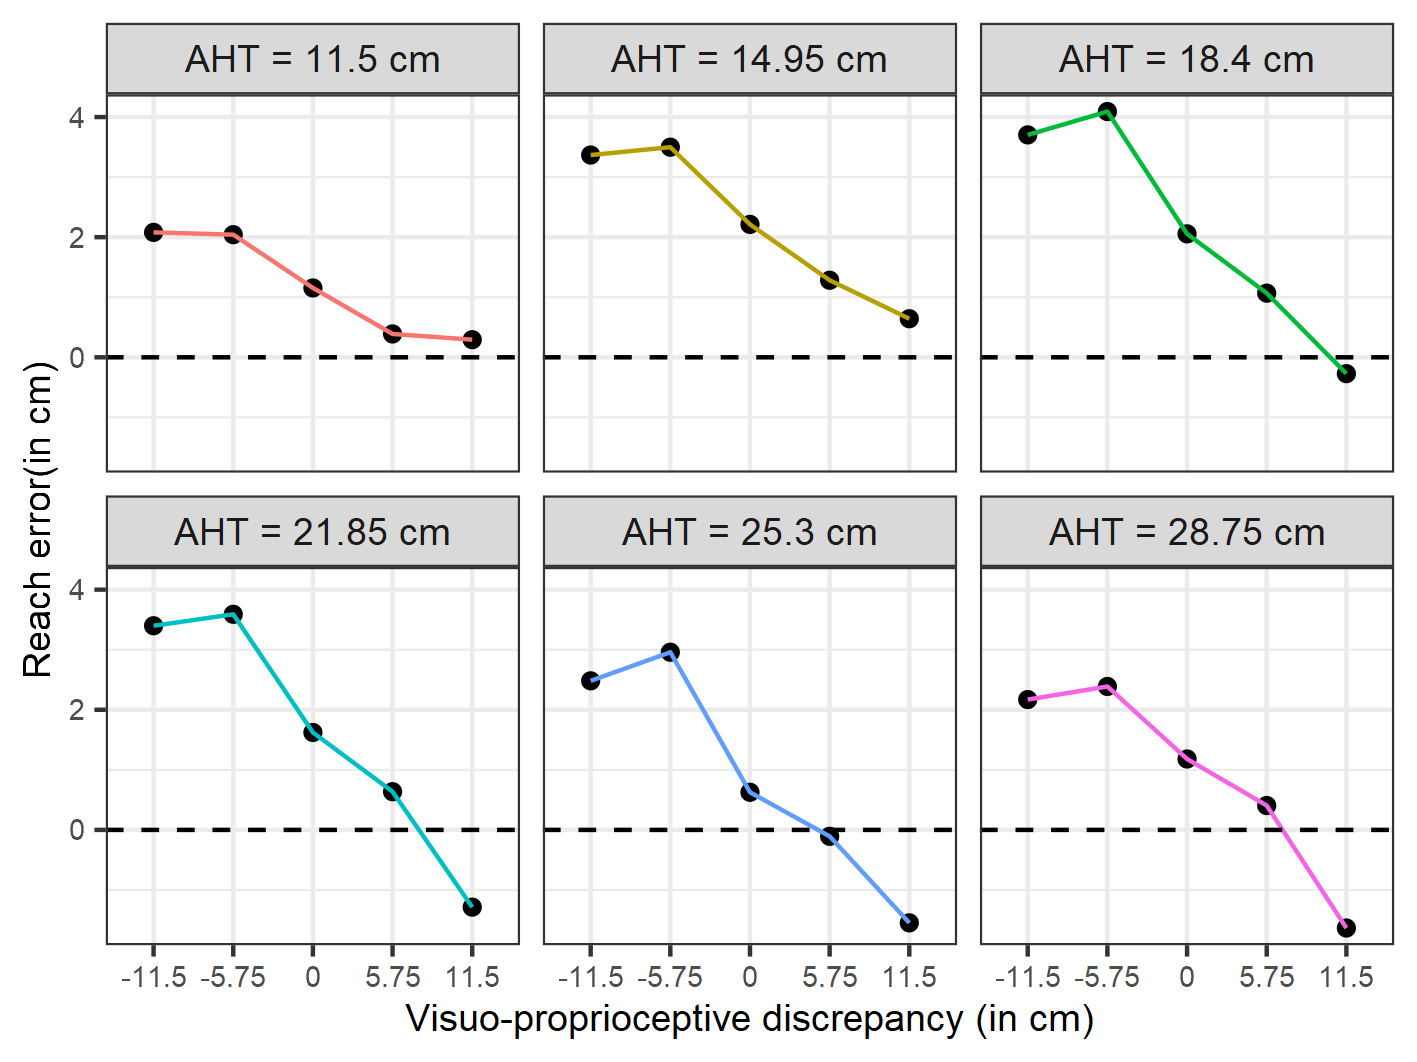
\includegraphics[scale=1]{Images/exp2_results2.png}
    \caption{Reach error as a function of spatial discrepancy between the position of visual hand and the position of actual (proprioceptive) non-action hand. Each panel shows the distance between the target and the initial position of the action hand (AHT). Negative reach error indicates that the estimation of the target location was in the direction of the non-action hand towards the left, while positive reach error indicates that the location of the target was estimated in the direction of action hand towards the right of the actual location of the target.}
    \label{fig:exp2_re-aht}
\end{figure}

Figure \ref{fig:exp2_re-aht} shows the effect of visuo-proprioceptive spatial discrepancy of proximal non-action hand on reach error, at different reach distances, that is, distance between the target and the initial position of the action hand. 

Since, the location of the proprioceptive signal is fixed according to the design of the experiment, the values of visuo-proprioceptive discrepancy also may be interpreted as different positions of the visual hand. The results in Figure \ref{fig:exp2_re-aht} show that there is a general underestimation (reach error is positive), when the target is closer to the action hand (Panel AHT = 11.5, 14.95, 18.4). However, as the visual hand is rendered closer to the target, the reach error decreases and the target estimation is more accurate. However, as the distance between the target and the action hand increases (Panels 21.85, 25.3, 28.75), the reach error is negative when the visual hand is rendered very close to the target (Discrepancy = +11.5cm). This suggests that it is not the accuracy that is improving as the visual hand is placed closer to the target, rather the estimate of the target's location is "pulled" towards the proximal non-action hand, as the distance between the visual hand and target decreases.

Overall, the results suggest that it is not the visuo-proprioceptive discrepancy itself that is affecting the target's location estimation, since that would have displayed a convex or a concave curve, with same magnitudes of discrepancy showing similar reach errors. Rather, the proximity of the visual hand to the target biases the estimation of the target in its direction, suggesting that the spatial encoding of the target may be with respect to the visual information of the body part in proximity.

These results seem to contradict the hypothesis that the spatial encoding of the target is with respect to the position of the body-part estimated as a result of multi-sensory integration inference mechanism. 

\subsection{Lack of support for Bayesian Causal Inference Mechanism}

The competing hypothesis that we will now consider is that the spatial information of the reach target is encoded with respect to the position of the proximal body-part which is estimated as a result of multi-sensory integration process. One of the models of multi-sensory integration is the \textit{Bayesian Causal Inference Model}. This model specifies how noisy uni-sensory signals are weighted based on the probability that the signals arose from the same source, and then integrated according to Bayesian Inference \cite{kording2007causal, meijer2020computational}. Previous literature suggests that this model can reasonably explain how position of the body part is estimated from noisy visual and proprioceptive signals \cite{noel2018peri, fossataro2020immersive}. We implemented the model similar to the implementation by \citeA{fossataro2020immersive} to estimate the position of the non-action hand from the visual and proprioceptive signal positions as specified by the experimental manipulations described in the above experiment.

According to the model, the uni-sensory information is modeled as a probability distribution, specifying the probability at all possible locations that the uni-sensory object is present at that particular location. In this implementation, the visual and the proprioceptive signals are assumed to follow a Gaussian distribution, centered at the veridical location of the signal (specified by the experimental manipulation), with variance indicative of the sensory noise. In our implementation, we set the value of visual precision (inverse of variance) as 0.97, and the value of proprioceptive precision as 2.1, on the basis of results found by \citeA{noel2018peri}. The third parameter of the model is $P_\pi$, which represents the "prior" beliefs that the visual and proprioceptive signals belong to the same source. We set the value of $P_\pi = 0.5$ in our implementation.

The complete model is specified as - 

\begin{align*}   
    P(hp | x_v, x_p) 
    &= \Sigma_{c=own,diff} P(hp | x_v, x_p, C = c) P(C = c | x_v,x_p ) \\ 
    &= P(hp | x_v, x_p, C = own) P(C = own | x_v,x_p ) \\
    &+ P(hp | x_v, x_p, C = diff) P(C = diff | x_v,x_p )
\end{align*}

where, $P(hp | x_v, x_p) $ is the probability of inferred location of the non-action hand, given the uni-sensory signals $x_v$ and $x_p$. $C=own$ refers to the situation where the source of the two signals is same, while $C=diff$ refers to the situation where the source of the two signals is different.  When $C=own$ , $P(hp | x_v, x_p, C = own)$ is the Gaussian posterior distribution, centered at the average of the uni-sensory signals, with a variance equal to the inverse of the sum of the precision of the uni-sensory signals. When $C=diff$ , $P(hp | x_v, x_p, C = diff)$ is the probability distribution relying only on proprioceptive signal - Gaussian centered at mean of proprioceptive signal, with the proprioceptive signal noise as its variance. The weighing factors $P(C = own | x_v,x_p )$ and $P(C = own | x_v,x_p )$ specify the probabilities that the two uni-sensory signals arise from the "own" hand or "different" sources conditional on the uni-sensory signals. 

\begin{figure}[t]
\centering       
    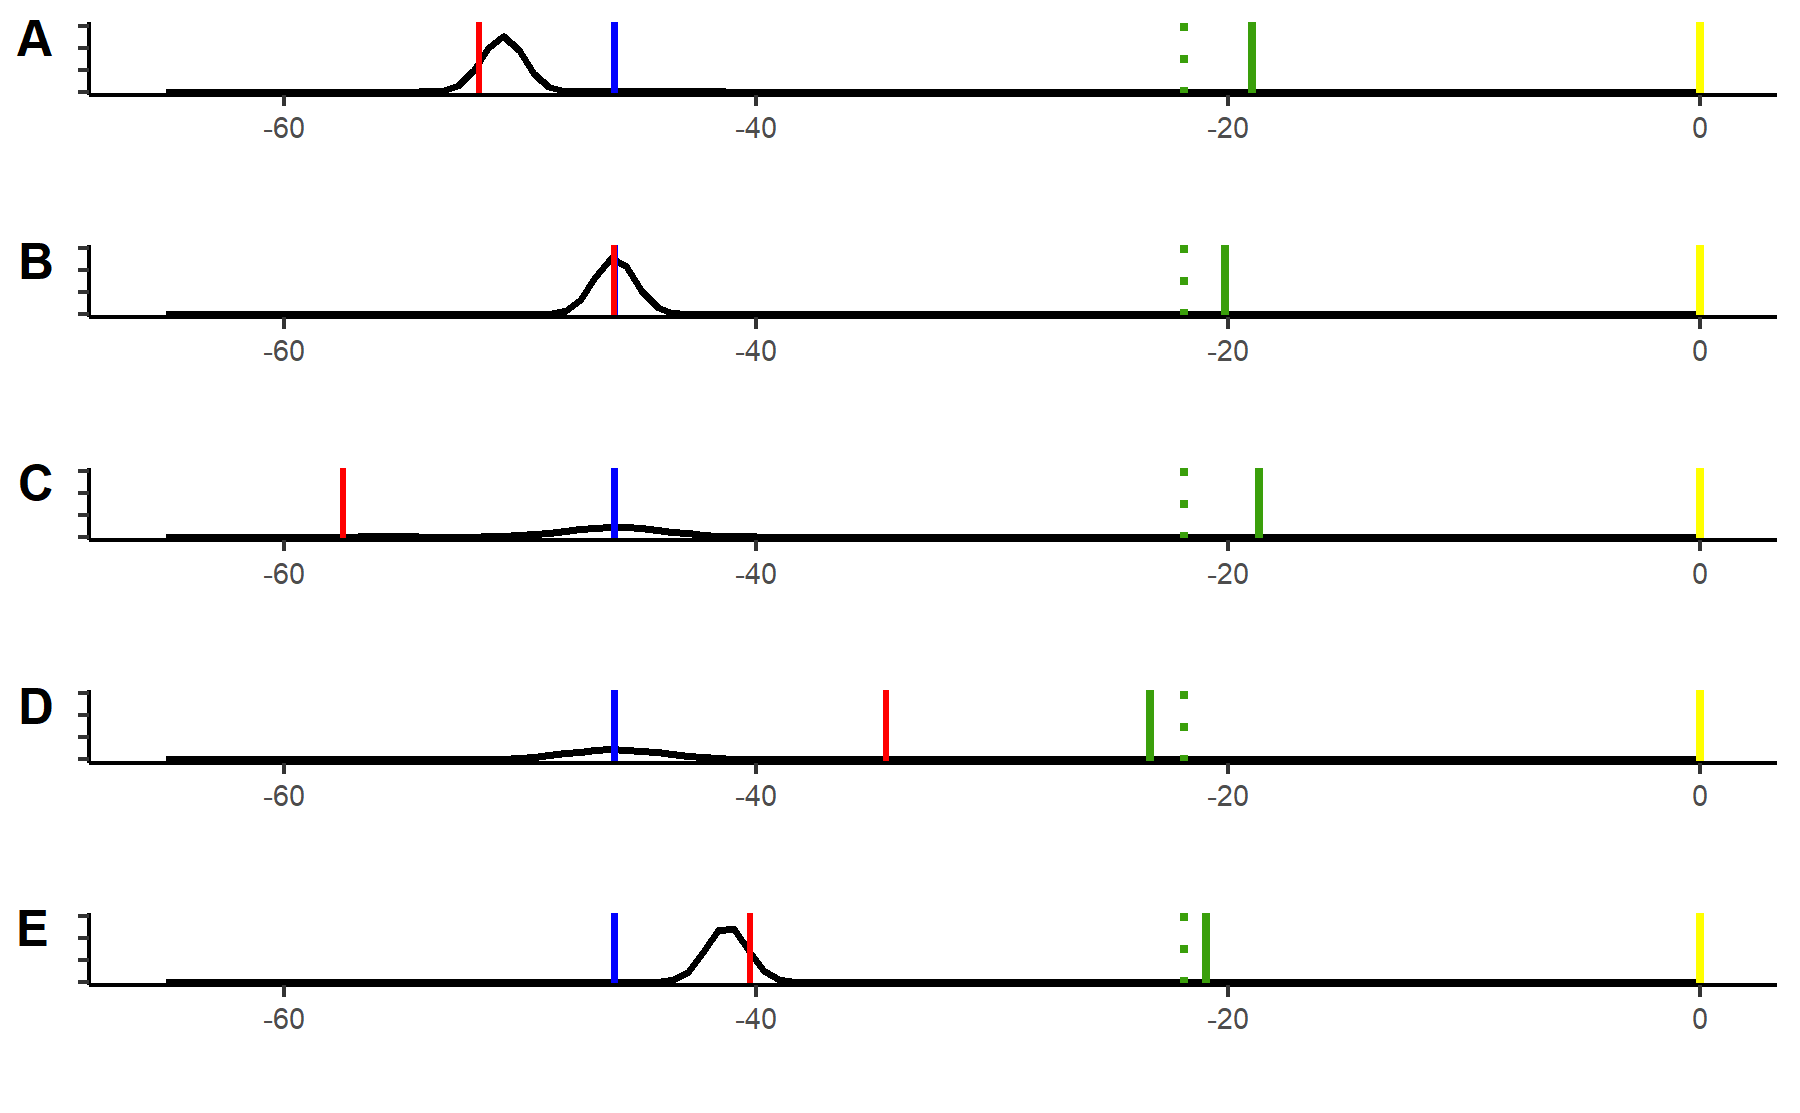
\includegraphics[width=\textwidth, keepaspectratio]{Images/bci_plot2.png}
    \caption{Estimated target location for Target Location = 21.85 cm, for different proximal hand's inferred positions according to the Bayesian Causal Inference Model. The red line indicates position of the visual signal of the proximal hand, while the blue line indicates the position of the proprioceptive signal, that is, the location of the placement of the real hand. The black curve indicates the probability density function denoting the probability of the location of the hand, as postulated by the multi-sensory integration process specified in the Bayesian Causal Inference Model. The mode of the distribution indicates the inferred position of the hand. The green dotted line indicates the veridical position of the reach target, while the solid green line indicates the (average) located estimated by the subjects. The yellow line indicates the initial position of the action hand. Panels A to E are ordered by the increasing proximity of the inferred hand position to the reach target, As seen in the figure, there is no systematic effect of proximity between the target and inferred hand position, and the target location estimation. }
    \label{fig:bci-plot2}
\end{figure}

We implemented this model to derive the probability distributions of non-action hand position at different levels of visuo-proprioceptive discrepancy. Figure \ref{fig:bci-plot2} shows these distributions with panels ordered according to the mode of the inferred hand position. Reach target veridical position at 21.85 cm from action hand and its average estimated position is also plotted (for other target positions, refer to Appendix \ref{App-bci-plots}). We observe that in the case of a high magnitude of visuo-proprioceptive discrepancy (Panel C and D, discrepancy = -11.5cm and +11.5cm), the mode of the inferred hand position is situated at the position of the proprioceptive hand. This is due to high probability attributed to the source of the uni-sensory signals being different (C = diff), due to the higher magnitude of spatial discrepancy between them. On the other hand, when the visuo-proprioceptive signals are relatively close (Panel A and E, discrepancy = -5.75cm and +5.75cm), we observe that the mode of the inferred hand position is shifted towards the visual hand. This is due to the high probability attributed to (C = own) and higher precision of visual signal. 

Qualitative inspection of the figure reveals that there is no systematic effect of the inferred position of the non-action hand on the reach target location estimation. In particular, consider Panel C and D. While the inferred position of the non-action hand is same in both cases, along with same uncertainty associated with the probability distribution, we observe differences in estimates for the reach target location. No systematic effect of inferred hand position is observed at other target positions as well (see Appendix \ref{App-bci-plots}). 

Therefore, the results of the experiment do not support the hypothesis that spatial encoding of the reach target occurs with respect to the inferred position of proximal body-part according to the Bayesian Causal Inference Model. On the other hand, the spatial encoding of reach target can be explained by encoding of the target's spatial information with respect to the visual signals of the proximal body-part, based on our results. 














\chapter{General Discussion} 
\label{discussion} 
\lhead{Chapter 5. \emph{General Discussion}} 

The purpose of this thesis was to investigate the following questions: i) Is the spatial information of the target of reach action represented with respect to body-part situated in its proximity, even if that body-part is not the effector involved in the reach action? ii) If yes, and considering that visuo-proprioceptive integration mechanism may underlie the construction of the representation of the body (\textit{body schema}), how is the integration of visual and proprioceptive signals specifying the spatial parameters of the proximal body-part involved in the spatial encoding of the reach target? To investigate these questions, we experimentally manipulated the presence of visual and proprioceptive information of a body-part proximal to the reach action target, and measured the accuracy of the target location estimated by the subjects in reaching action. 

The results of Experiment 1 show that when a body part is present proximal to the target, the target location estimation is more accurate, compared to the situation in which the body-part is not present proximal to the target. This result thus supports the hypothesis that spatial information of the target is indeed represented in an egocentric reference frame, with respect to the body-part proximal to the target. Thus, our finding confirms the results from previous literature that the objects in peri-personal space (here, the reach targets) are spatially encoded in a somatotopic (body-part centric) frame of reference \cite{serino2019peripersonal}. Notably, we have shown that this hypothesis is further supported through the paradigm of accuracy of reaches, and not merely through the paradigm of multi-sensory interaction effects, that has been a norm in the literature (See Chapter \ref{Literature Review}).

However, the target location estimation is not improved significantly when only uni-sensory information (visual or proprioceptive) about the proximal body-part is present. This is a significant finding, because it suggests that it is more merely the presence of a visual allocentric landmark that is affecting the target location estimation. Rather, the accuracy in target location estimation is improved only when multi-sensory visuo-proprioceptive signals of proximal body part are present. This suggests that visuo-proprioceptive multi-sensory integration mechanism plays a role in the spatial encoding of the reach target. This contradicts the results from various studies that show that presence of visual landmarks improves reaching performance \cite<e.g.>{krigolson2007proximity}; \cite<For review, see>{filimon2015all}. However, these studies used memory guided reach paradigm, instead of invisible action-hand reach paradigm to induce variability in the reaches. It is possible that memory-guided reaches have another (allocentric) mechanism underlying the reach target spatial encoding. 

\citeA{fossataro2020immersive} showed that when there is high visuo-proprioceptive discrepancy of a body-part, the peri-personal space as operationalized by the magnitude of multi-sensory interactions, enlarges, suggesting that since the estimation of body-part position (according to Bayesian Casual Inference) is less precise due to the high visuo-proprioceptive discrepancy, peri-personal space is enlarged to optimize reactions to external events. Particularly, their findings show that the magnitude of multi-sensory interaction effects are comparable when the visual stimuli occurs near to the proprioceptive or the visual signal of the body part. Our results contradict \citeA{fossataro2020immersive}'s finding that the inference of body-part position affecting the spatial encoding of visual objects in peri-personal space. When visuo-proprioceptive spatial discrepancy is induced in the proximal body-part, the results of the experiment show that the estimation of the target is "pulled" towards the proximal body-part as a function of proximity of the target to the visual signal. This finding suggests that although the results from the previous experiment suggest that a body-part proximal multi-sensory integration mechanism underlies the spatial encoding of the target, the spatial encoding itself seems to occur with respect to the visual signal regarding the proximal body-part. Furthermore, we implemented the Bayesian Causal Inference Model to estimate the inferred location of the proximal body-part based on inputs from the spatially discrepant visual and proprioceptive signals. These inferred proximal body-part positions do not systematically explain the reach errors measured in the experiment. Thus, our results do not support the hypothesis that the reach target is spatially encoded with respect to the position of the proximal body-part as inferred from a multi-sensory integration process by an ideal Bayesian observer. 

The discrepancies between the results may be due to the difference in the paradigms implemented in the two studies. In our experiment, we implemented a localization of visual stimuli in peri-personal space paradigm, while \citeA{fossataro2020immersive} implemented a multi-sensory interaction effects paradigm which is based on reaction times. It is plausible that the spatial properties attributed to the multi-sensory interaction effects observed in peri-personal space and the the spatial encoding of objects in peri-personal space may have different conceptual and mechanistic basis. Indeed, \citeA{bufacchi2021peripersonal} have discussed the idea that there is not a single peri-personal space representation, rather, a set of responses arising in the space surrounding the body, which may be indicative of distinct cognitive processes. 

Overall, our novel findings are i) Multi-sensory visuo-proprioceptive information of the proximal body part may be necessary for the spatial encoding of reach target to occur with respect to it, however ii) the encoding may occur with respect to the visual signal, as opposed to the inferred position of the proximal body-part estimated by an Ideal Bayesian observer. There are however several limitations of our study which must be acknowledged. Firstly, there are some intrinsic limitations in our experimental design. The distance between proprioceptive signal and the target (which keeping the distance between the action hand and target constant) has been been systematically manipulated, which prevents us from making stronger claims regarding the spatial encoding of the target with respect to the proprioceptive signal. Secondly, in our study, the Bayesian Causal inference Model has been implemented to get predictions regarding the inferred body-part position according to an ideal Bayesian observer, and reach responses are compared for different levels of proximity of inferred body-part position to the reach target. While our results and analysis merely point towards the probable multi-sensory mechanism, a stronger case can be made if the reach error itself can be modeled in the Bayesian Causal Inference framework, while experimentally determining the parameters for the model. 

In summary, the findings from our work suggest that a proximal body-part's visuo-proprioceptive multi-sensory integration mechanism underlies the spatial encoding of reach target, and that the spatial encoding occurs with respect to the visual information before integration with the proprioceptive information, however, further empirical investigation is required to substantiate this  claim.











%APPENDICES

\addtocontents{toc}{\vspace{2em}} 

\appendix 
\chapter{Experiment 1: Data Analysis} 
\label{App-exp1-analysis} 
\lhead{Appendix A. \emph{Experiment 1: Data Analysis}} 

\section{Assumptions of Repeated Measures ANOVA}

\begin{table}[H]
\centering
\begin{tabular}{rlrrl}
  \hline
 & Effect & W & p & p$<$.05 \\ 
  \hline
1 & block & 0.90 & 0.87 &  \\ 
  2 & sti\_pos & 0.25 & 0.00 & * \\ 
  3 & block:sti\_pos & 0.14 & 0.02 & * \\ 
   \hline
\end{tabular}
\caption{Mauchly's Test for Sphericity}
\label{}
\end{table}

\begin{table}[H]
\centering
\resizebox{\textwidth}{!}{
\begin{tabular}{rlrlrlrlrl}
  \hline
 & Effect & GGe & DF[GG] & p[GG] & p[GG]$<$.05 & HFe & DF[HF] & p[HF] & p[HF]$<$.05 \\ 
  \hline
1 & block & 0.94 & 2.81, 56.17 & 0.02 & * & 1.10 & 3.31, 66.29 & 0.02 & * \\ 
  2 & sti\_pos & 0.57 & 1.14, 22.89 & 0.00 & * & 0.58 & 1.17, 23.37 & 0.00 & * \\ 
  3 & block:sti\_pos & 0.60 & 3.62, 72.38 & 0.23 &  & 0.75 & 4.52, 90.35 & 0.22 &  \\ 
   \hline
\end{tabular}}
\caption{Spericity Corrections}
\label{}
\end{table}

\section{Post-hoc Analysis Results}

\begin{table}[H]
\centering
\begin{tabular}{rlllrrrrrrl}
  \hline
 & .y. & group1 & group2 & n1 & n2 & statistic & df & p & p.adj & p.adj.signif \\ 
  \hline
1 & avg\_mre & L & C &  21 &  21 & 2.06 & 20.00 & 0.05 & 0.05 & ns \\ 
  2 & avg\_mre & L & R &  21 &  21 & 3.22 & 20.00 & 0.00 & 0.01 & ** \\ 
  3 & avg\_mre & C & R &  21 &  21 & 3.73 & 20.00 & 0.00 & 0.00 & ** \\ 
   \hline
\end{tabular}
\caption{Pair-wise t test between levels of Target Position. Adjusted P-values are Holm-Bonferroni corrected.}
\end{table}



\begin{table}[H]
\centering
\resizebox{\textwidth}{!}{
\begin{tabular}{rlllrrrrrrl}
  \hline
 & .y. & group1 & group2 & n1 & n2 & statistic & df & p & p.adj & p.adj.signif \\ 
  \hline
1 & avg\_mre & X & PV &  21 &  21 & 2.94 & 20.00 & 0.01 & 0.05 & * \\ 
  2 & avg\_mre & PV & P &  21 &  21 & -2.55 & 20.00 & 0.02 & 0.10 & ns \\ 
  3 & avg\_mre & PV & V &  21 &  21 & -1.51 & 20.00 & 0.15 & 0.59 & ns \\ 
  4 & avg\_mre & V & P &  21 &  21 & -1.32 & 20.00 & 0.20 & 0.61 & ns \\ 
  5 & avg\_mre & X & V &  21 &  21 & 1.31 & 20.00 & 0.20 & 0.41 & ns \\ 
  6 & avg\_mre & X & P &  21 &  21 & -0.14 & 20.00 & 0.89 & 0.89 & ns \\ 
   \hline
\end{tabular}}
\caption{Pair-wise t test between levels of Visuo-proprioceptive information of Non-action hand. Adjusted P-values are Holm-Bonferroni corrected.}
\end{table}
\input{Appendices/Experiment-2-Analysis.tex}
\chapter{Bayesian Causal Inference Model Estimates} 
\label{App-bci-plots} 
\lhead{Appendix C. \emph{Bayesian Causal Inference Model Estimates}} 

The plots in this appendix show the predictions of proximal hand's inferred positions according to the Bayesian Causal Inference Model, along with the estimated target locations (measured experimentally) for different target locations.

The red line indicates position of the visual signal of the proximal hand, while the blue line indicates the position of the proprioceptive signal, that is, the location of the placement of the real hand. The black curve indicates the probability density function denoting the probability of the location of the hand, after multi-sensory integration process postulated by the Bayesian Causal Inference Model. The mode of the distribution indicates the inferred position of the hand. The green dotted line indicates the veridical position of the reach target, while the solid green line indicates the (average) located estimated by the subjects. The yellow line indicates the initial position of the action hand. Panels A to E are ordered by the increasing proximity of the inferred hand position to the reach target.


\begin{figure}[h]
\centering       
    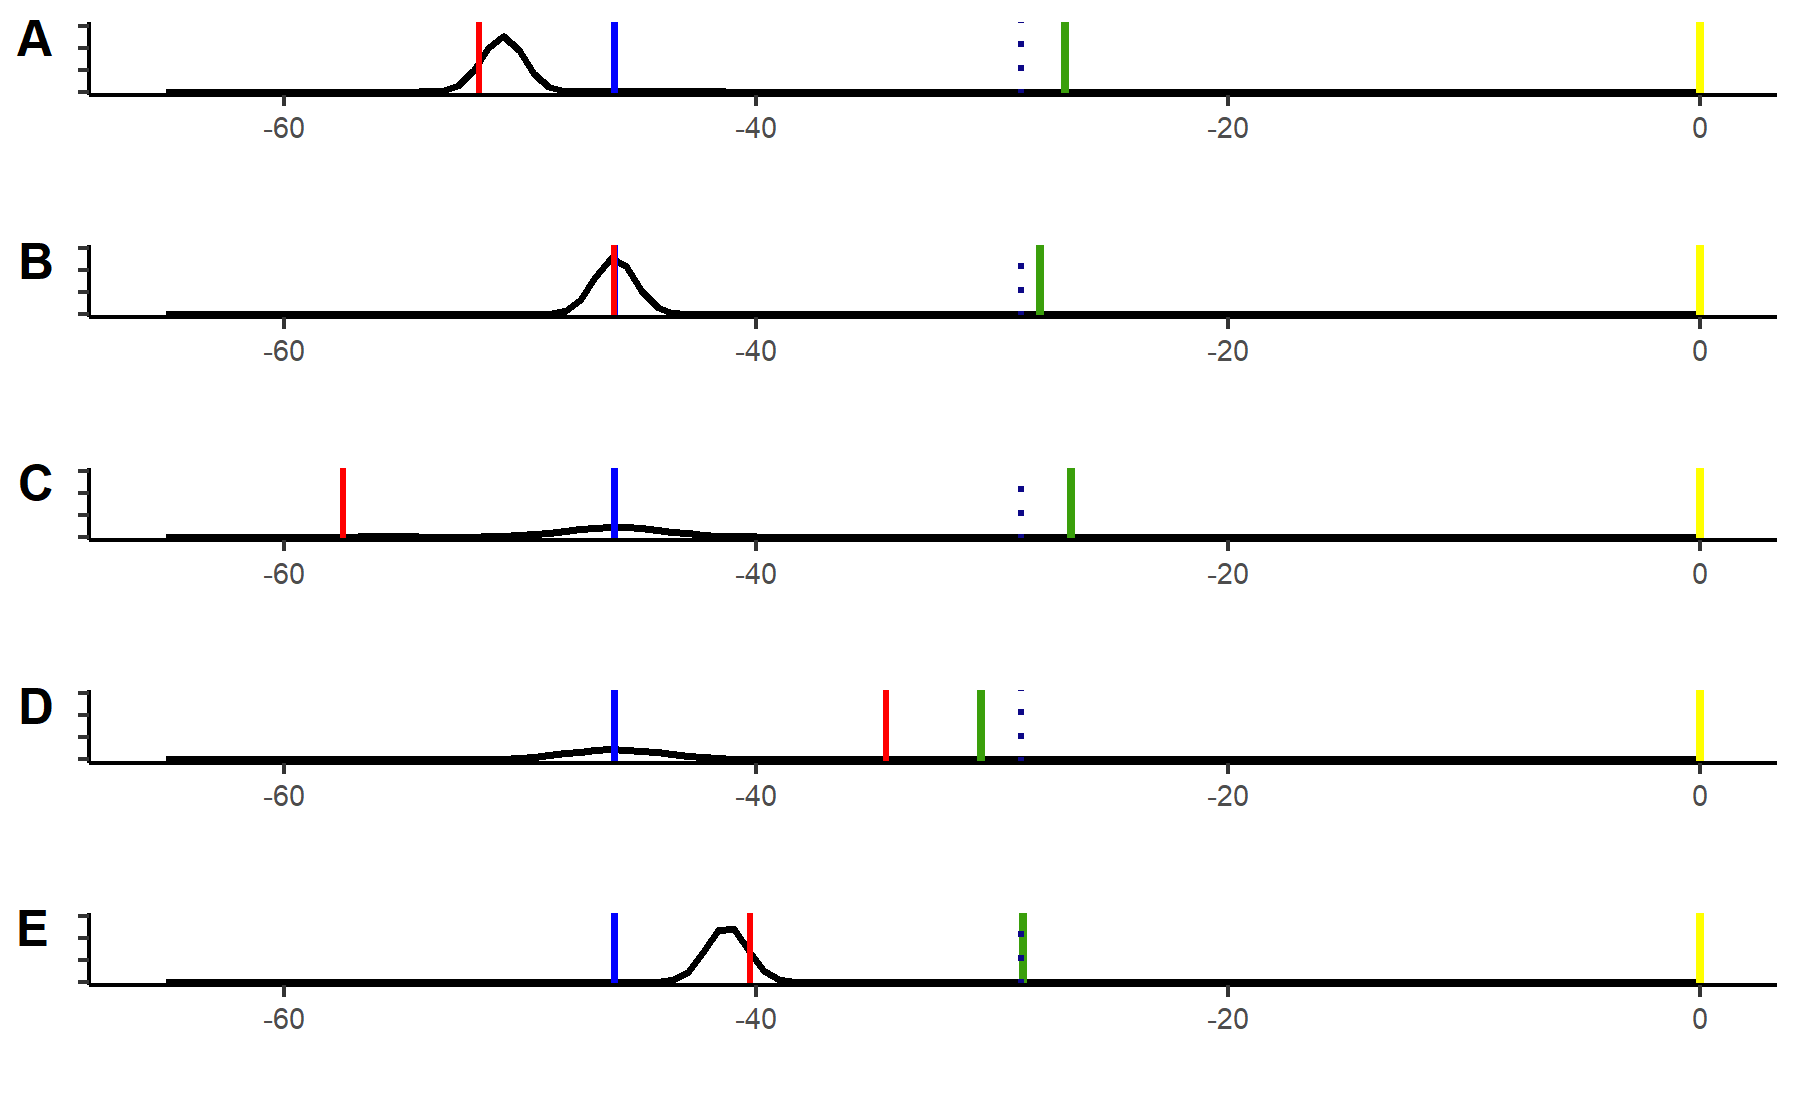
\includegraphics[width=\textwidth, keepaspectratio]{Images/bci-plots/bci_plot17-25.png}
    \caption{Target Location = 28.75 cm}
    \label{}
\end{figure}

\begin{figure}[h]
\centering       
    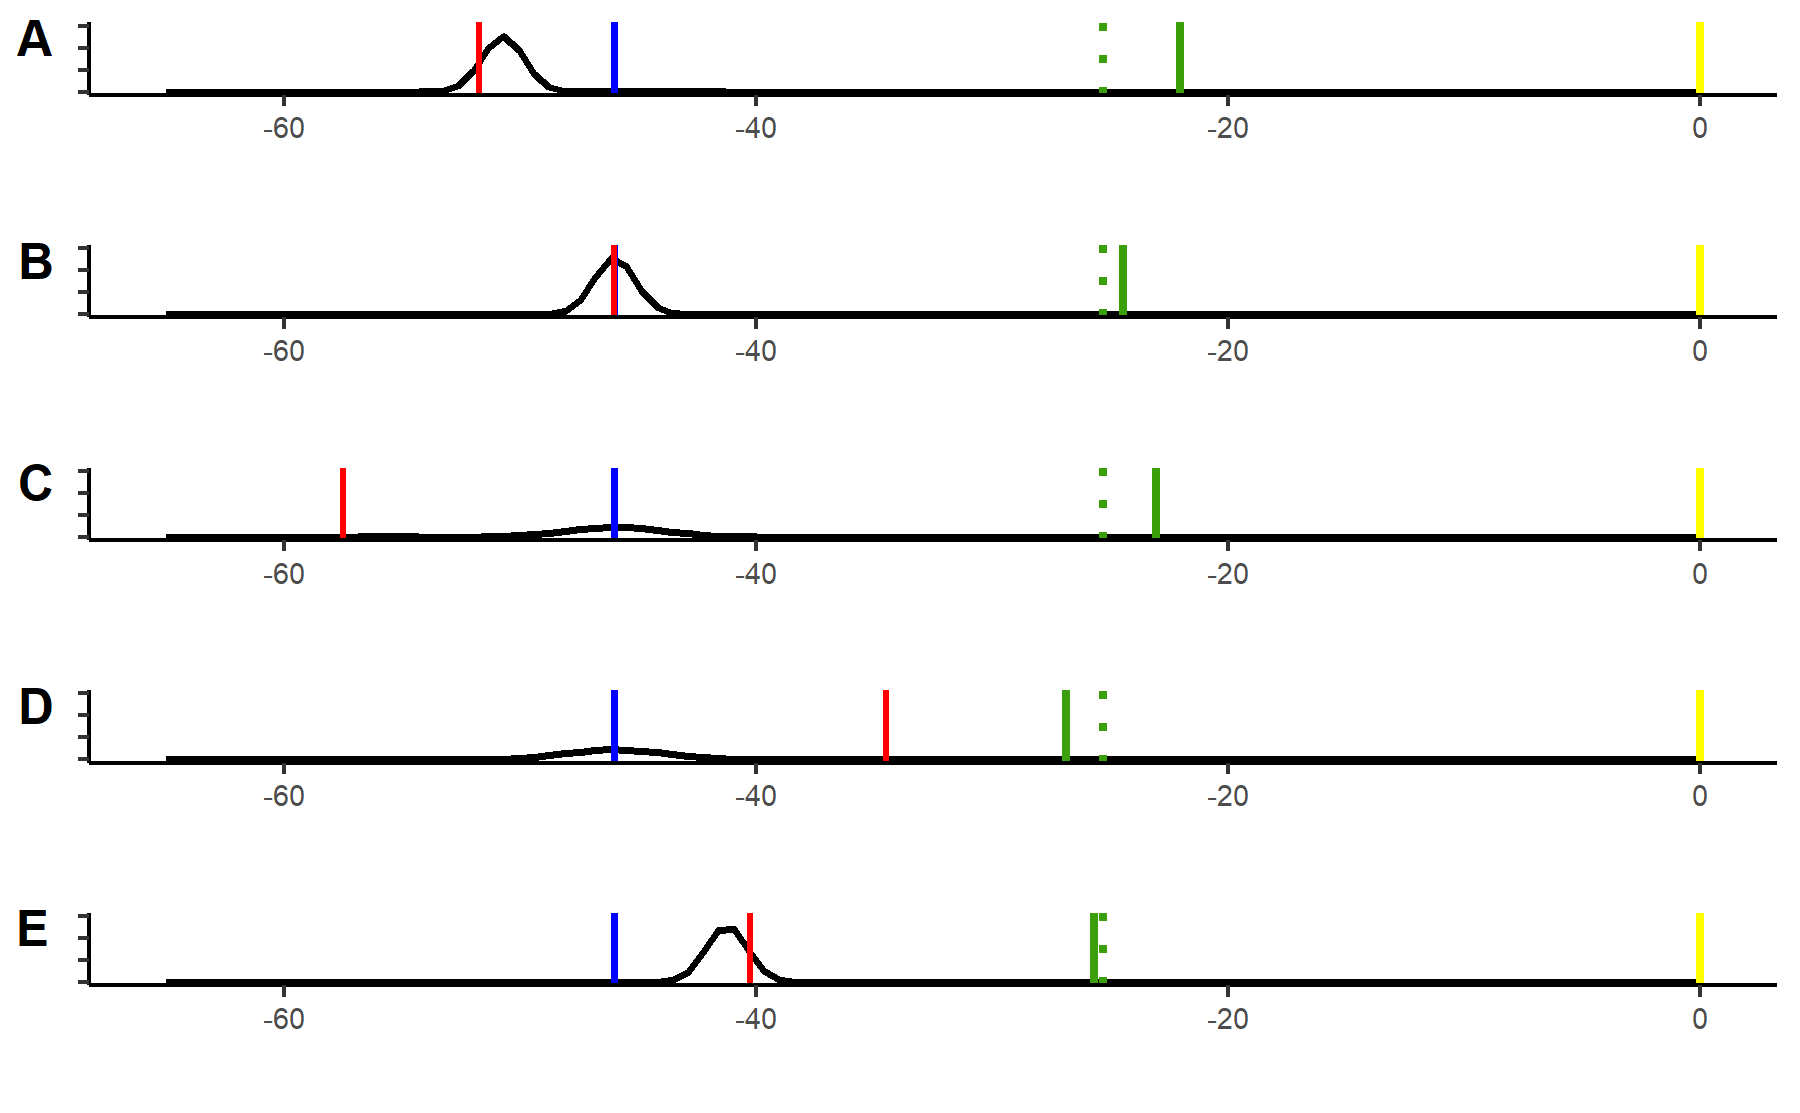
\includegraphics[width=\textwidth, keepaspectratio]{Images/bci-plots/bci_plot20-7.png}
    \caption{Target Location = 25.3 cm}
    \label{}
\end{figure}

\begin{figure}[h]
\centering       
    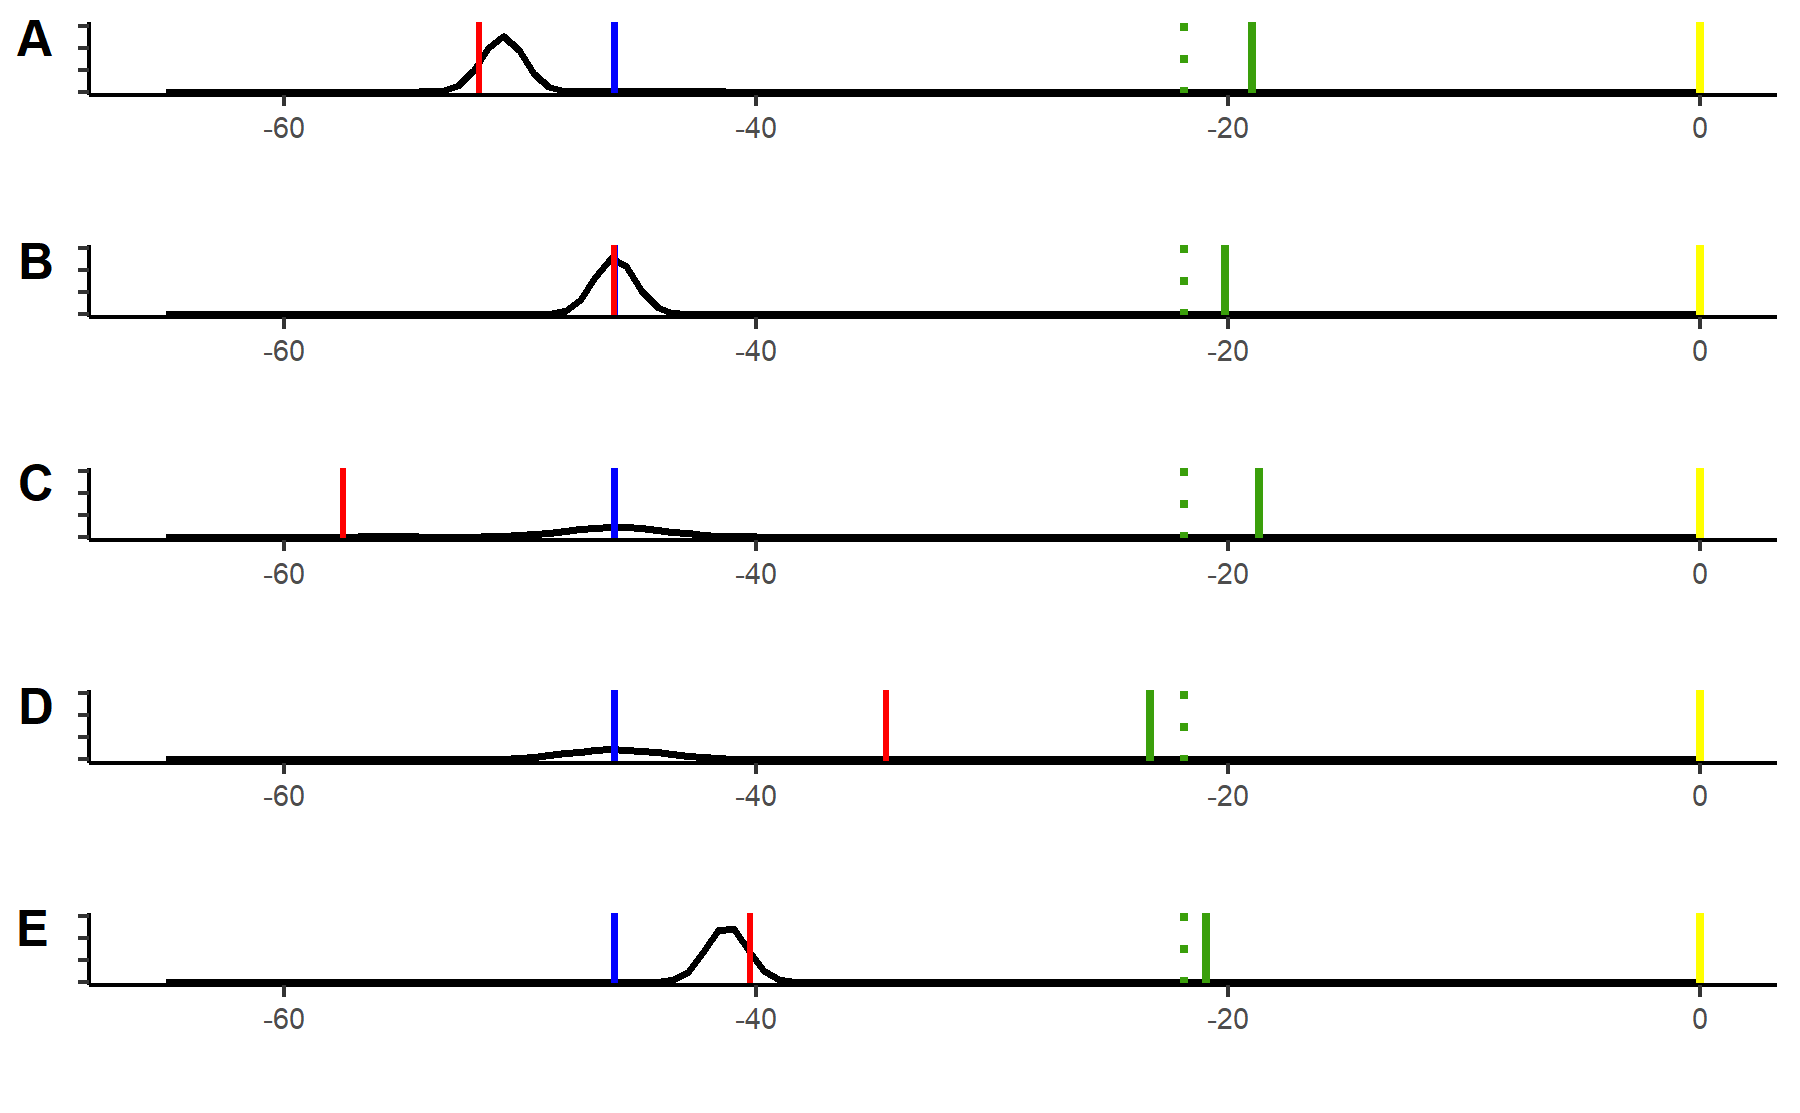
\includegraphics[width=\textwidth, keepaspectratio]{Images/bci-plots/bci_plot24-15.png}
    \caption{Target Location = 21.85 cm}
    \label{}
\end{figure}

\begin{figure}[h]
\centering       
    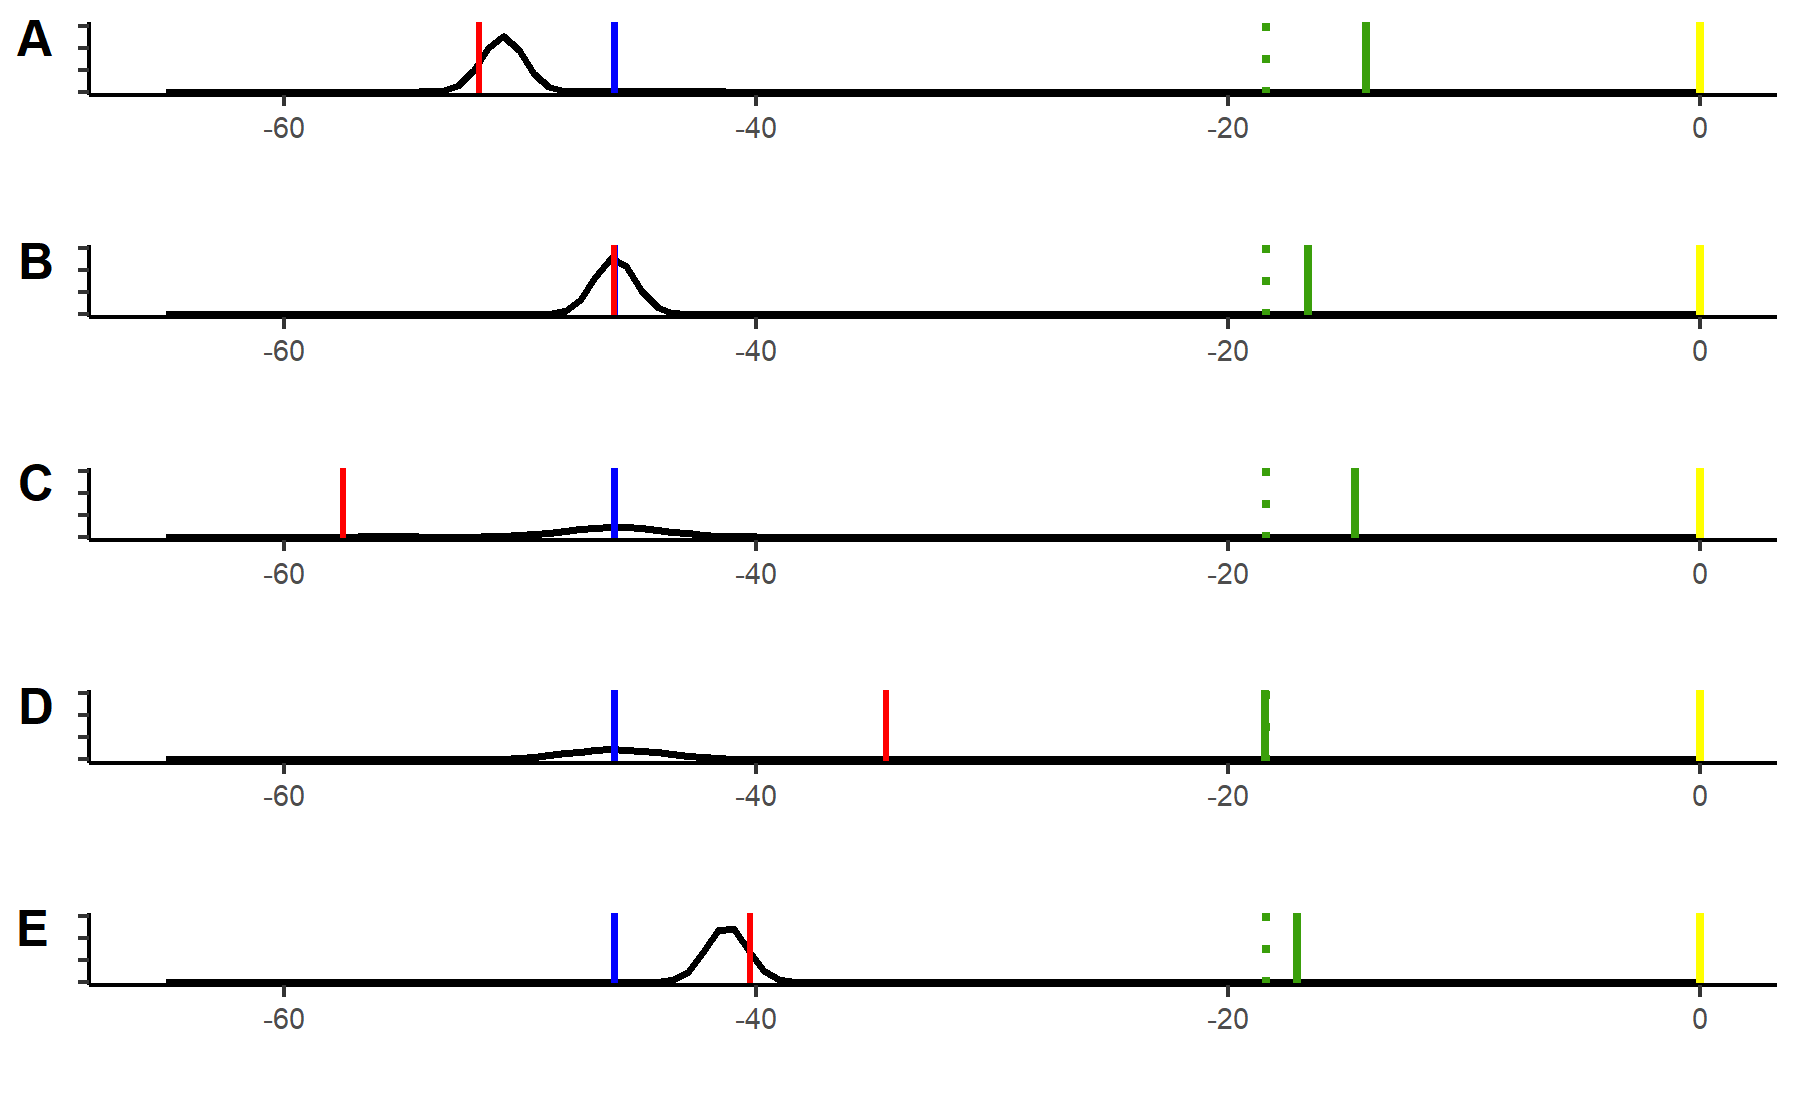
\includegraphics[width=\textwidth, keepaspectratio]{Images/bci-plots/bci_plot27.6.png}
    \caption{Target Location = 18.4 cm}
    \label{}
\end{figure}

\begin{figure}[h]
\centering       
    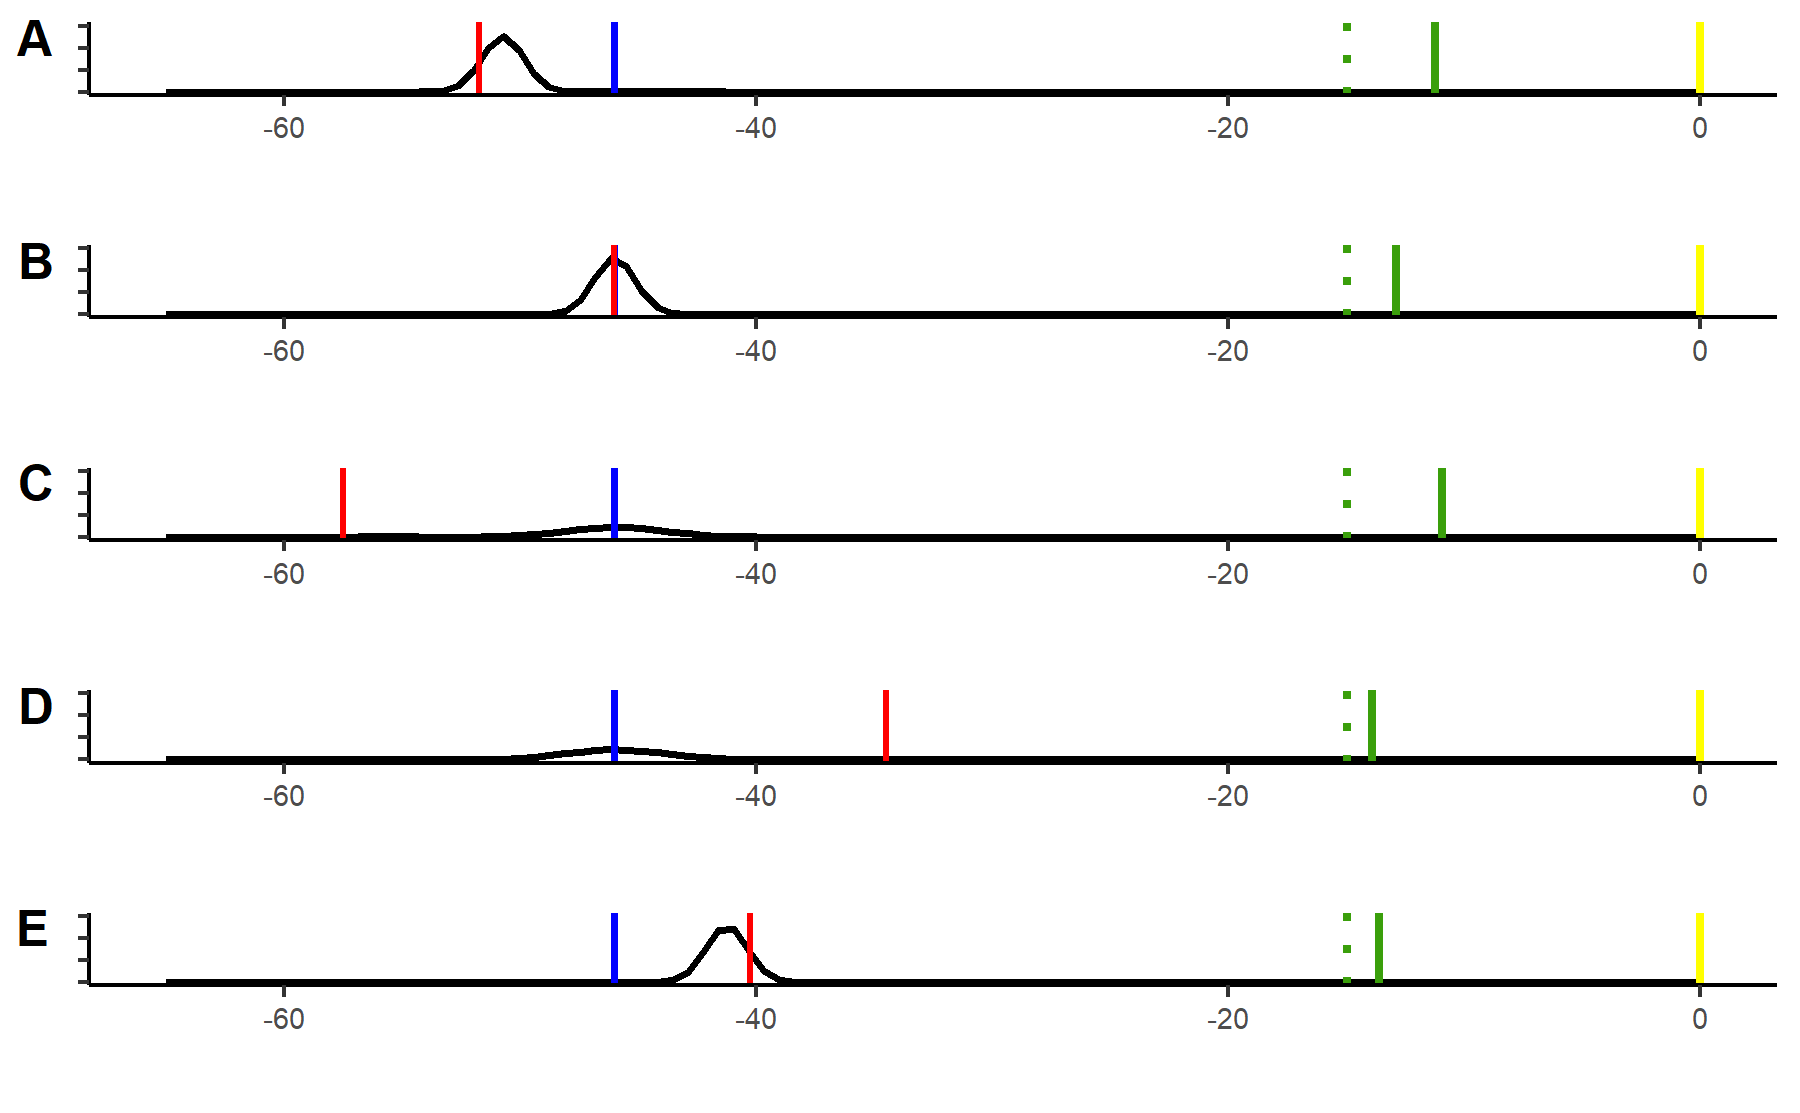
\includegraphics[width=\textwidth, keepaspectratio]{Images/bci-plots/bci_plot31-05.png}
    \caption{Target Location = 14.95 cm}
    \label{}
\end{figure}

\begin{figure}[h]
\centering       
    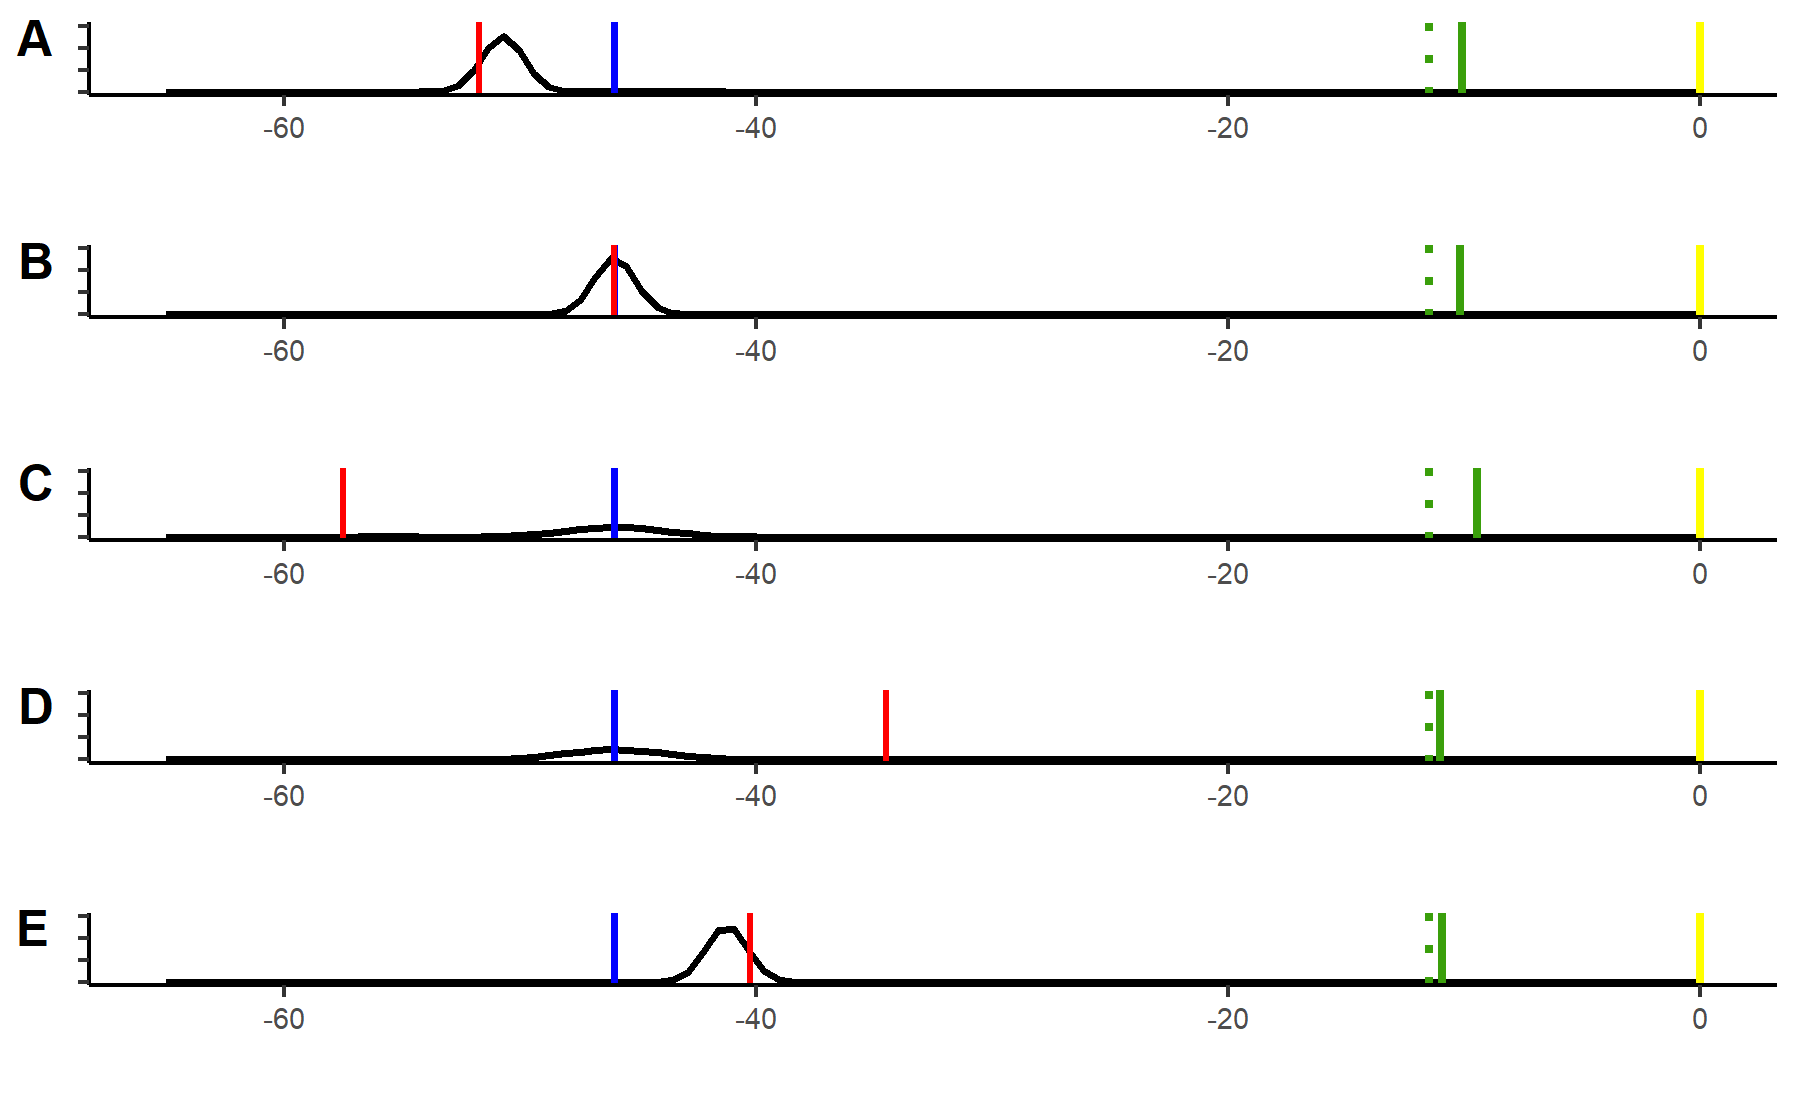
\includegraphics[width=\textwidth, keepaspectratio]{Images/bci-plots/bci_plot34-5.png}
    \caption{Target Location = 11.5 cm}
    \label{}
\end{figure}
\chapter{Instructions and Consent Documents} 
\label{App-vr-disclaimer} 
\lhead{Appendix D. \emph{Instructions and Consent Documents}} 

\begin{figure}[h!]
\centering  
    \caption{Experiment 1: Instructions}
    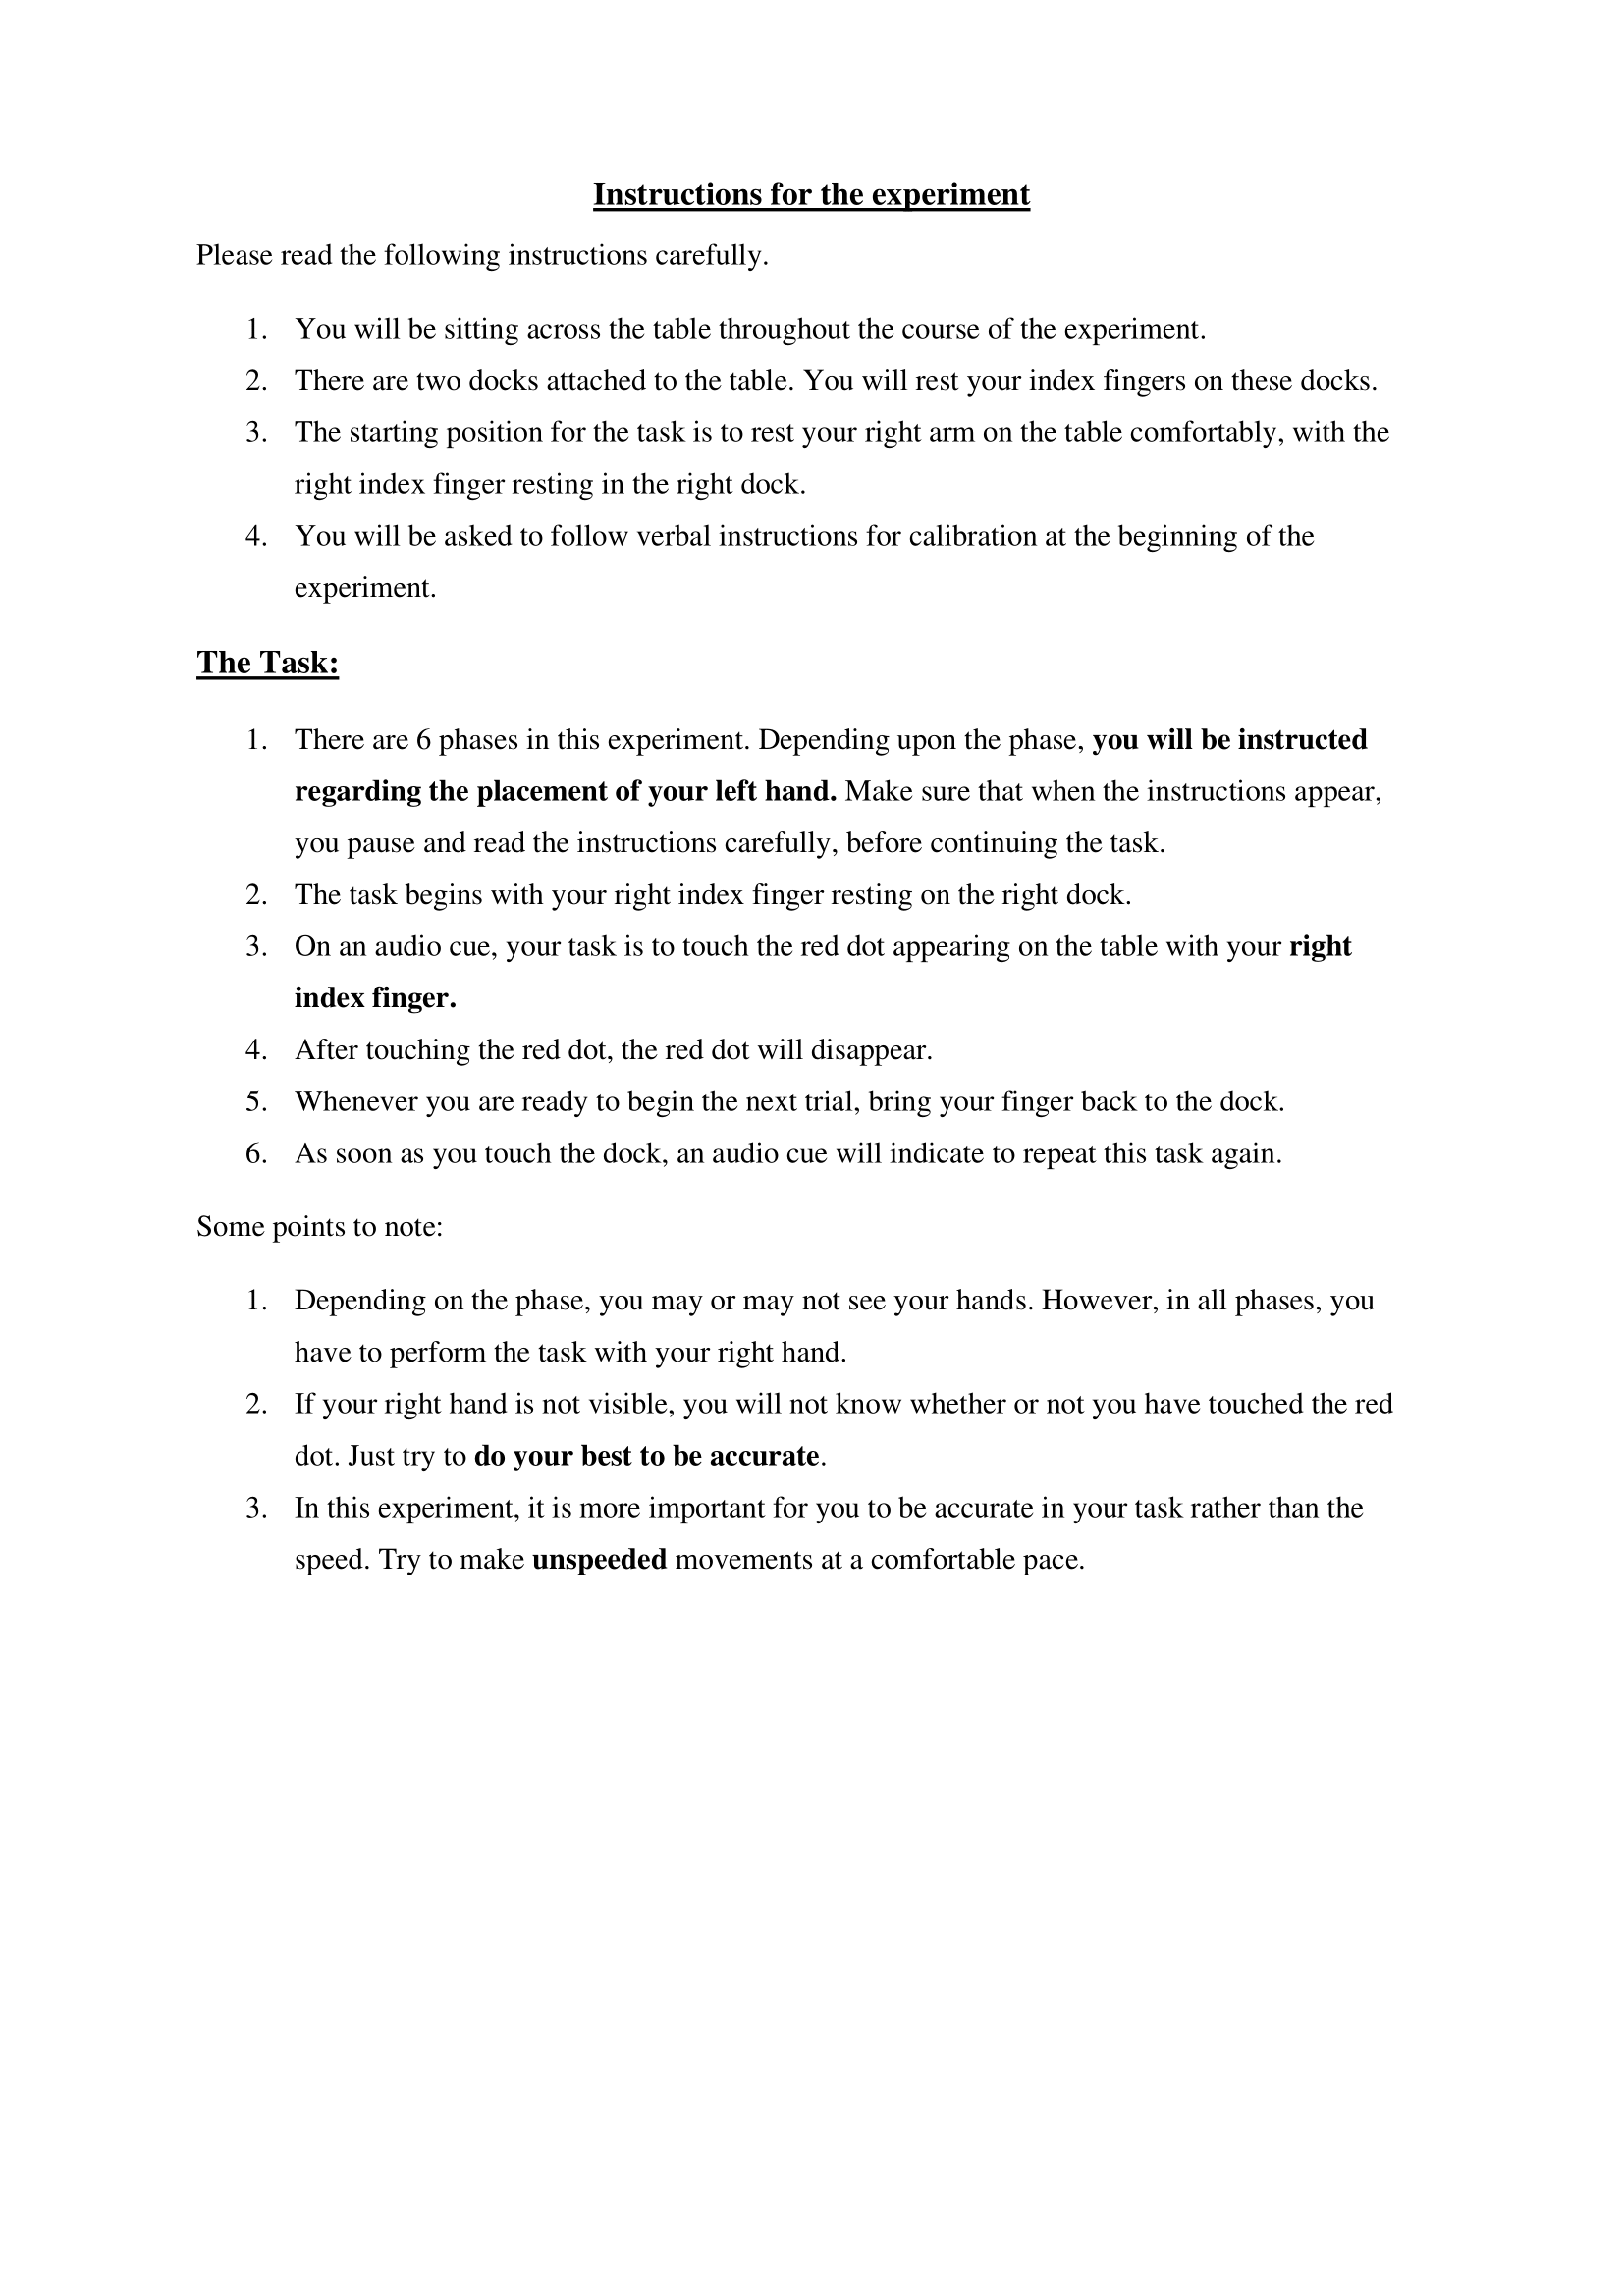
\includegraphics[width=\textwidth, keepaspectratio]{Images/admin/exp1-instructions.png}
    \label{}
\end{figure}

\begin{figure}[h!]
\centering       
    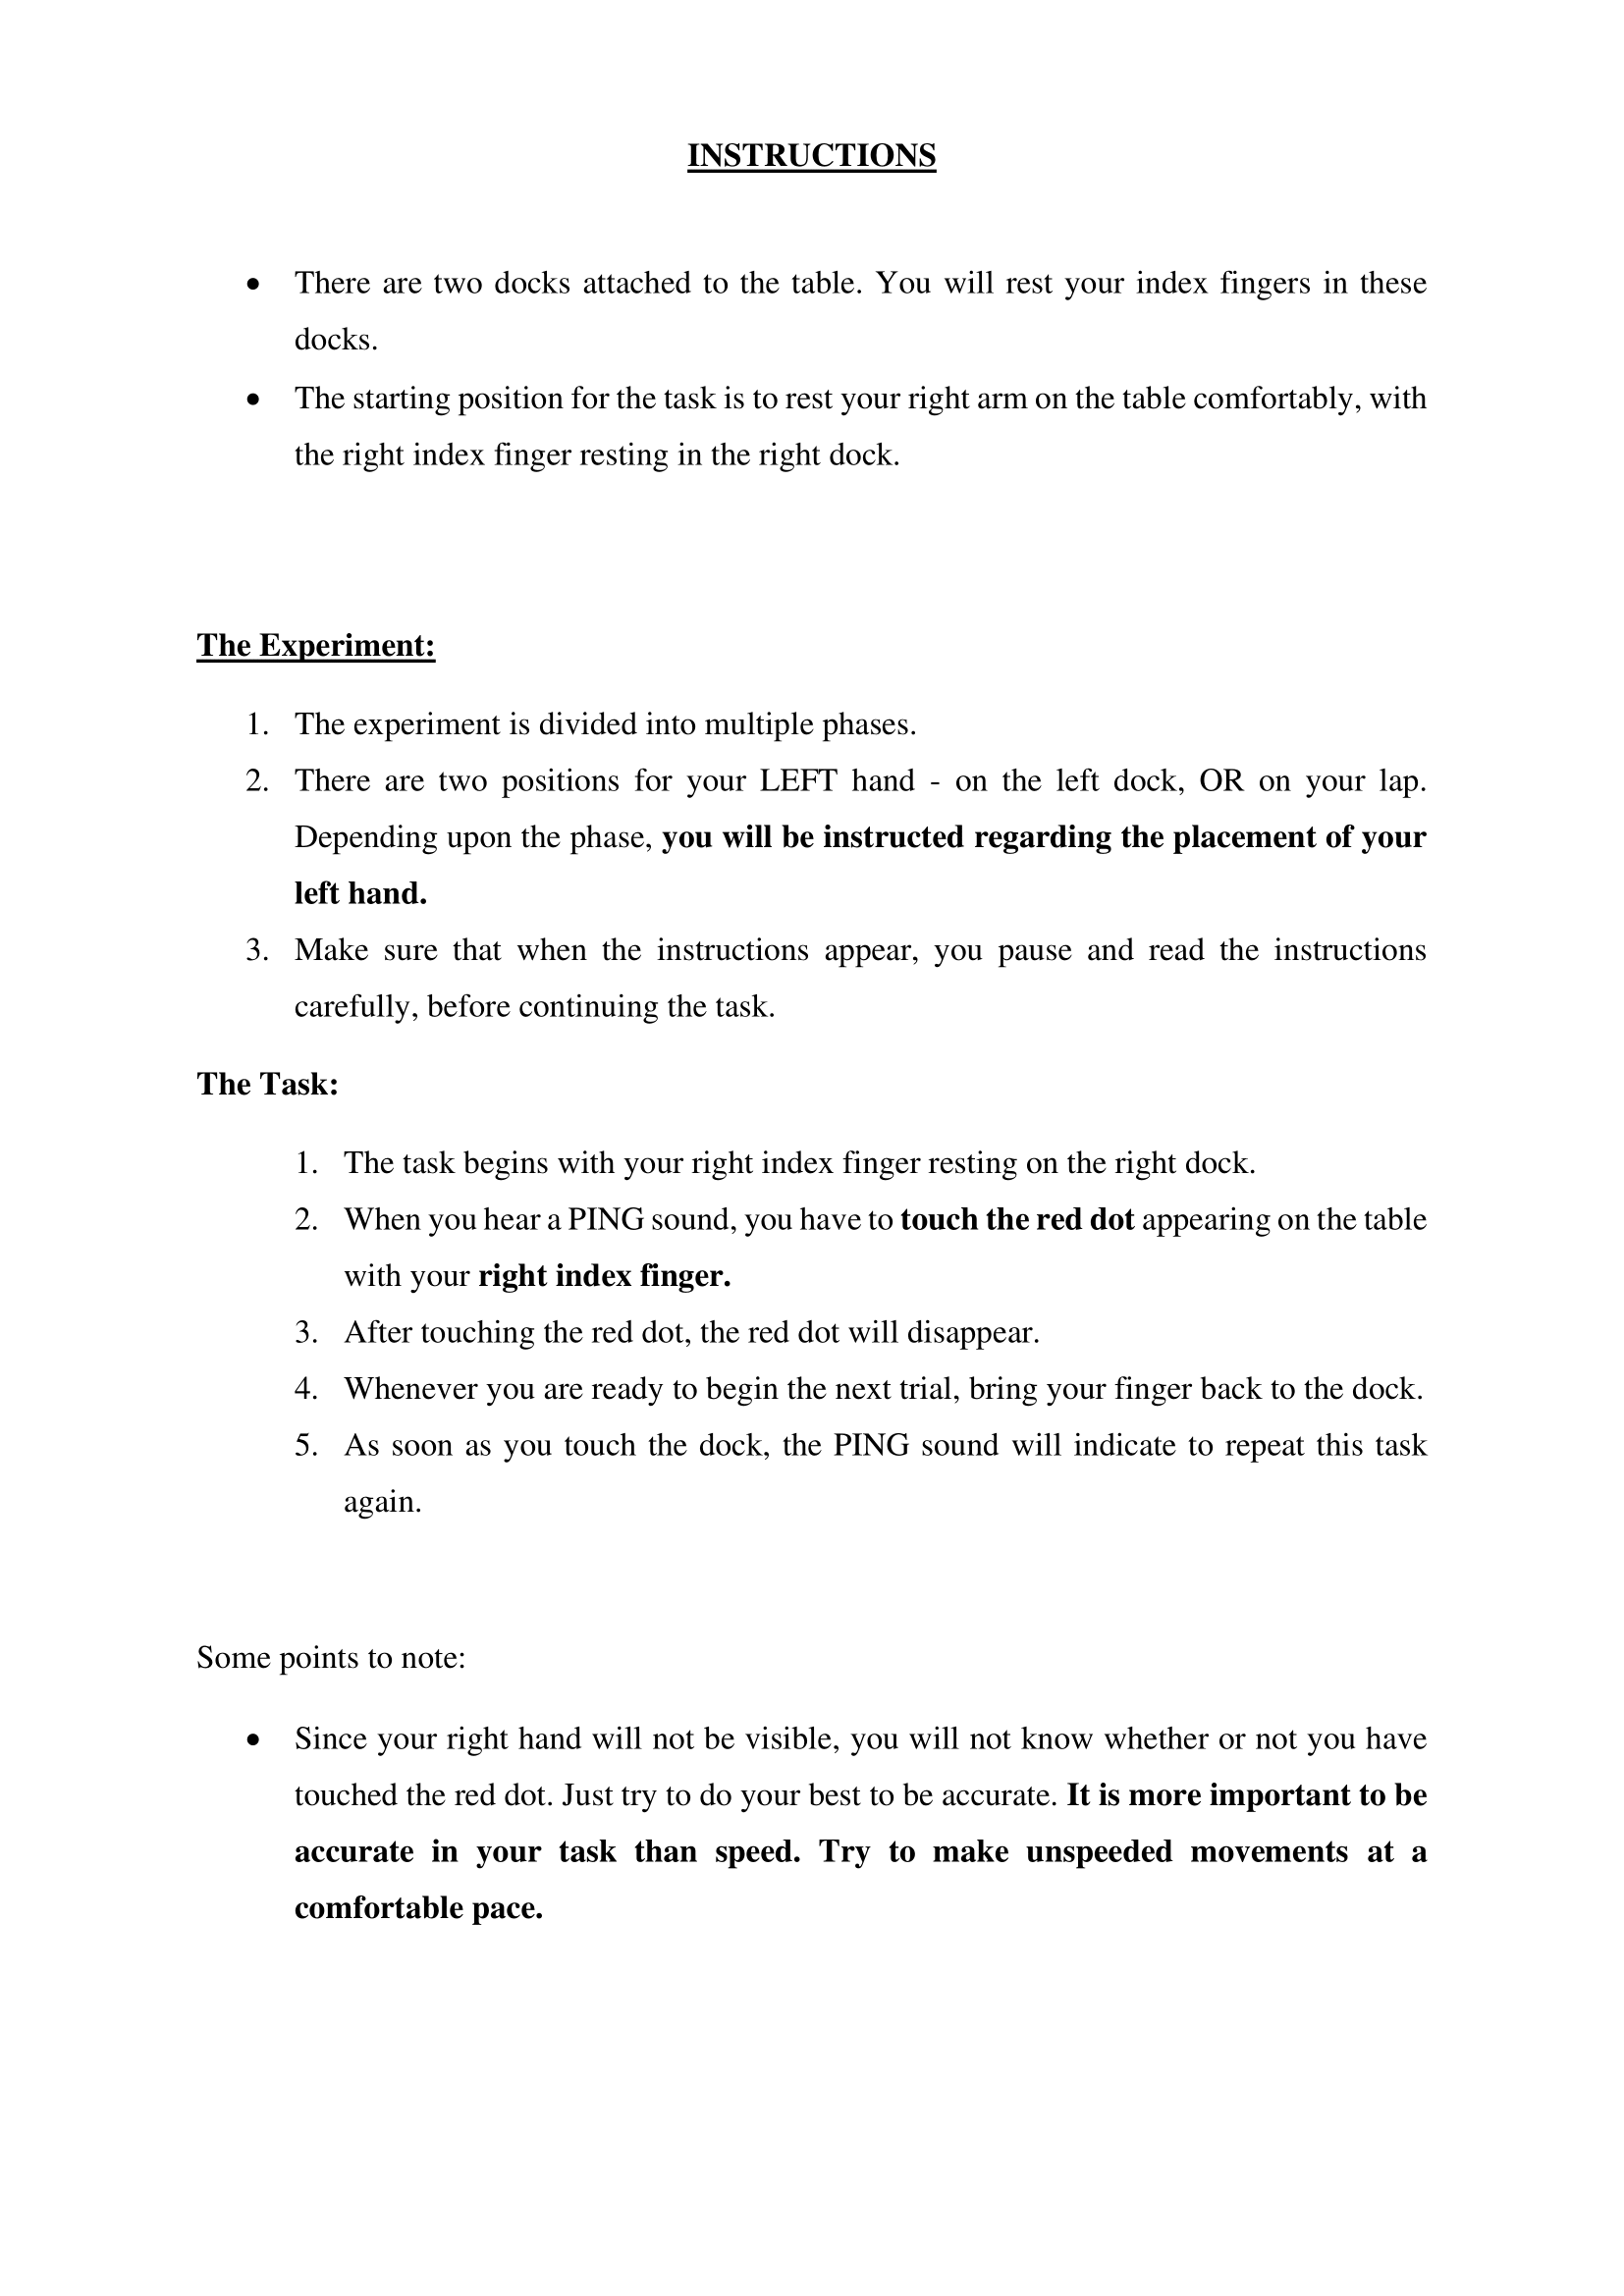
\includegraphics[width=\textwidth, keepaspectratio]{Images/admin/Exp2- Instructions-1.png}
    \caption{Experiment 2: Instructions}
    \label{}
\end{figure}

\begin{figure}[h!]
\centering       
    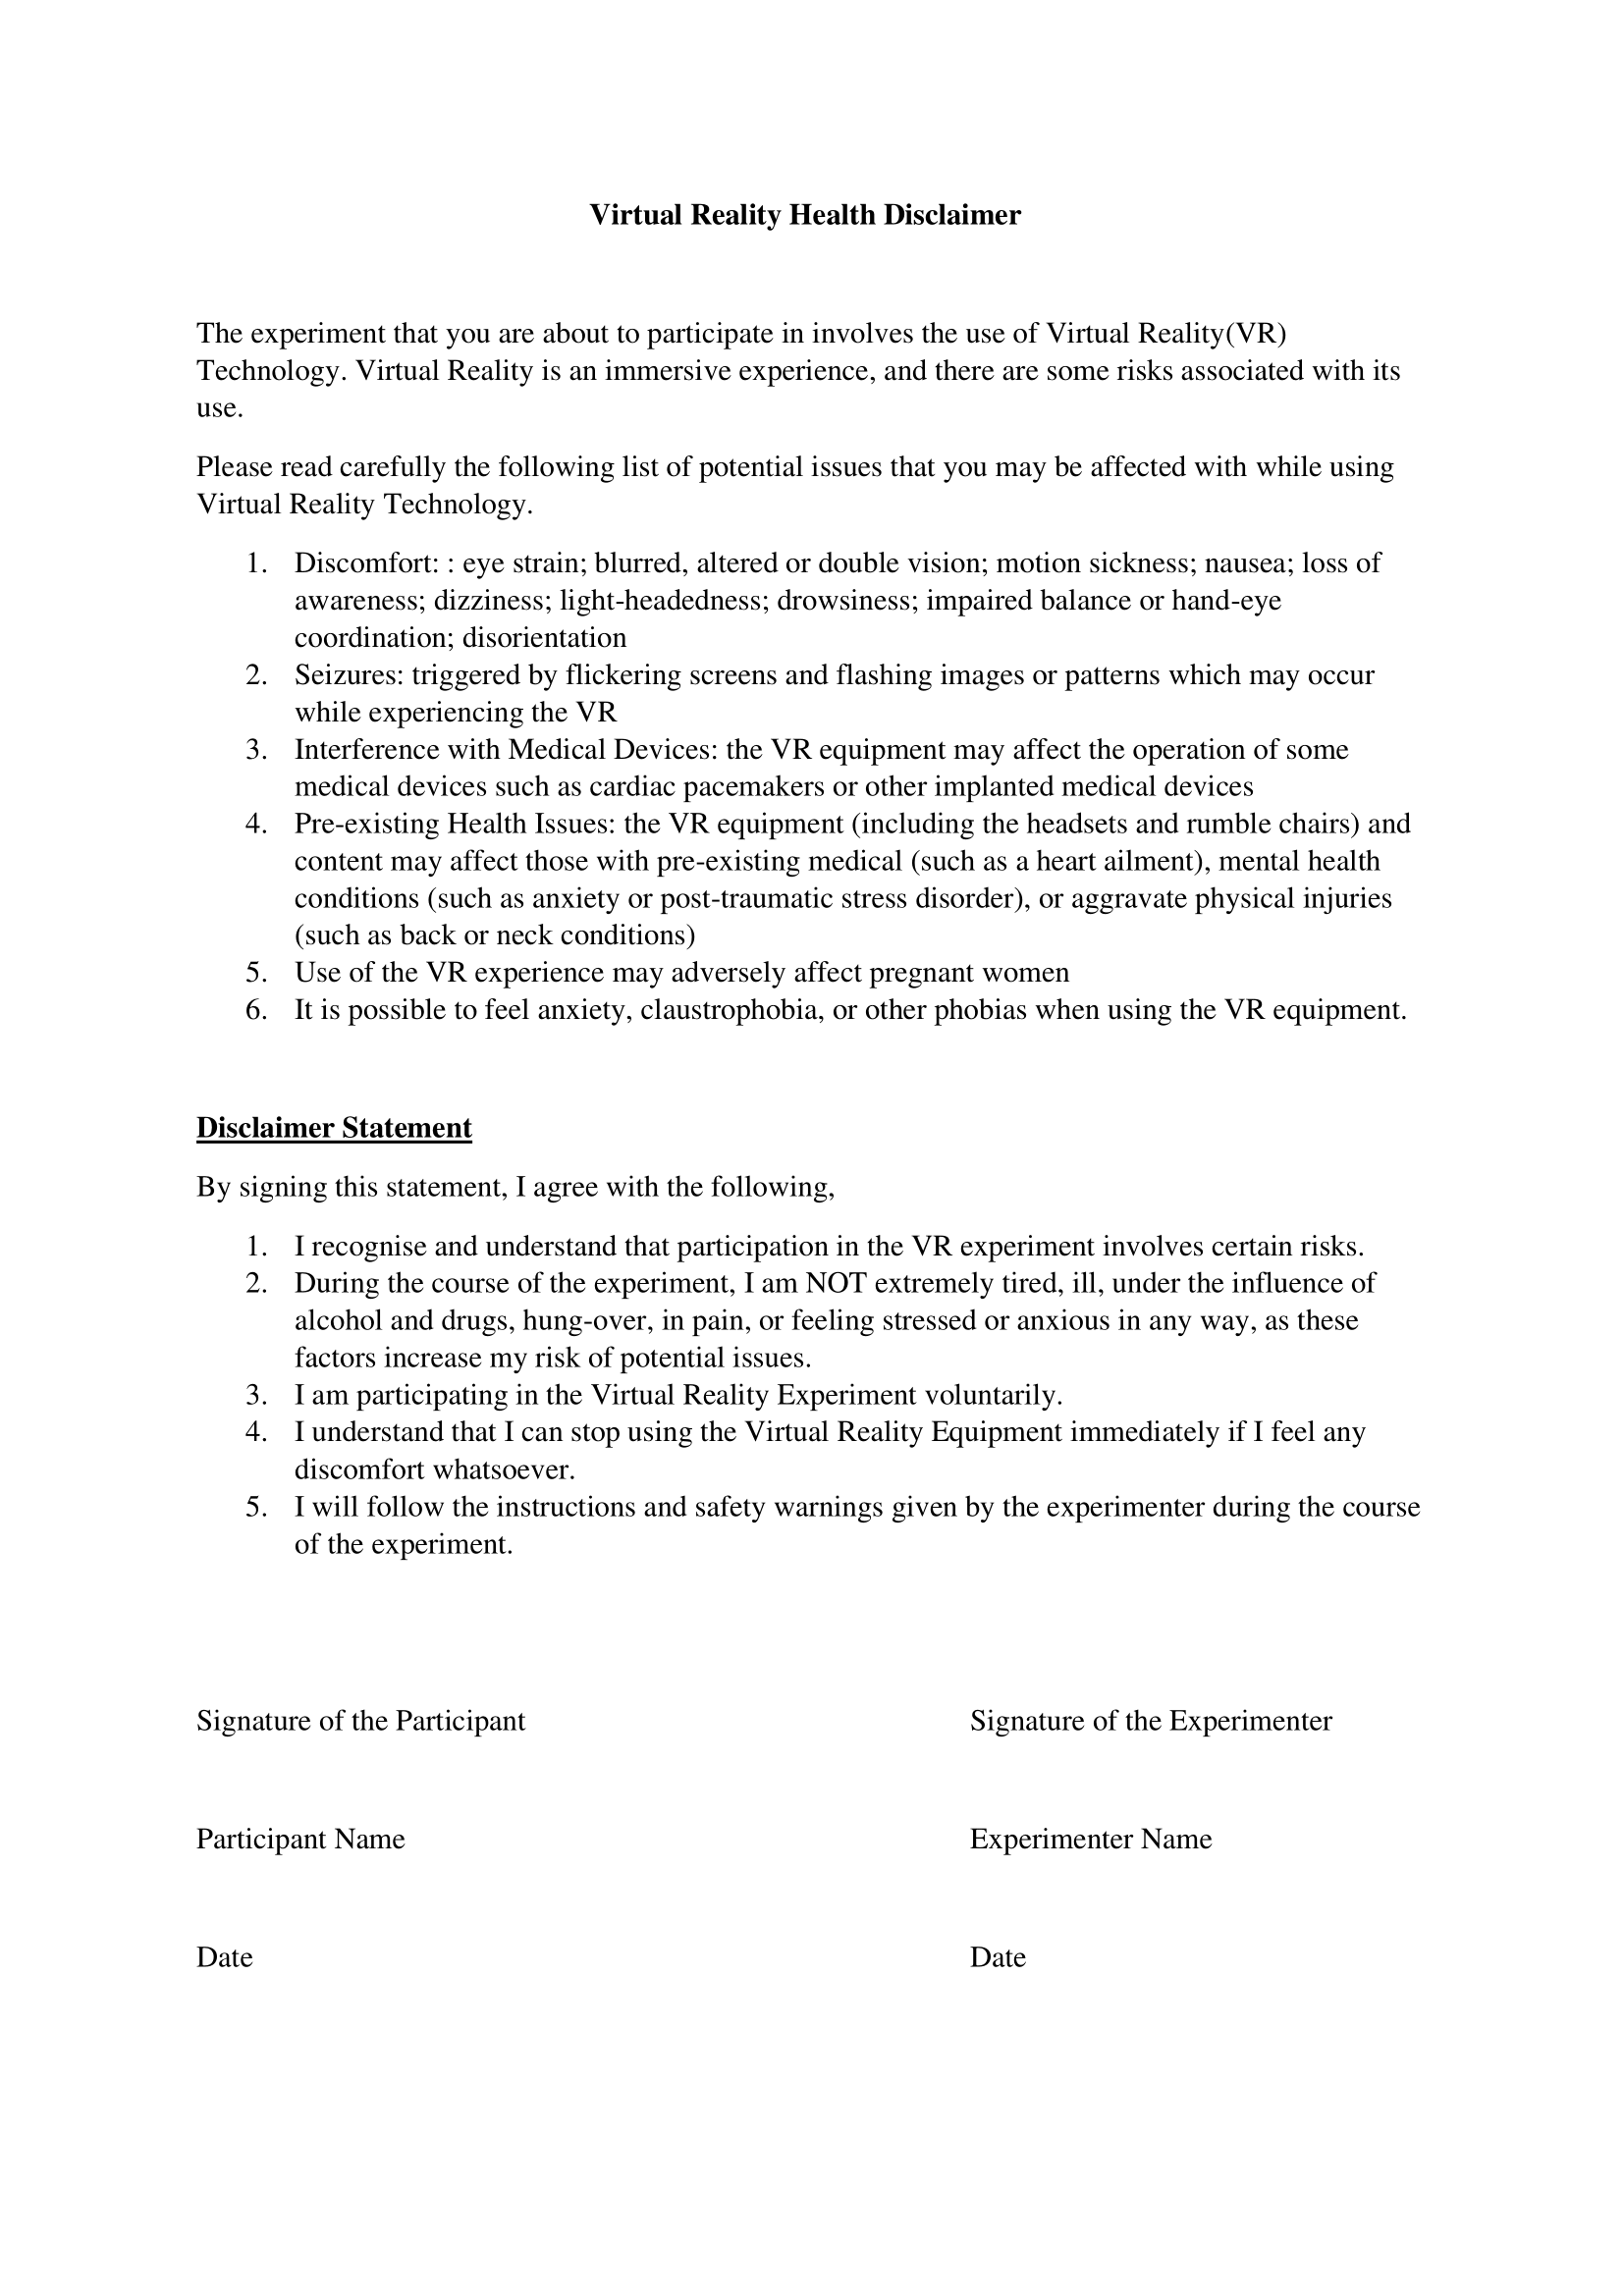
\includegraphics[width=\textwidth, keepaspectratio]{Images/admin/Virtual Reality Health Disclaimer- Updated-1.png}
    \caption{ Virtual Reality Health Disclaimer}
    \label{}
\end{figure}

\begin{figure}[h!]
\centering       
    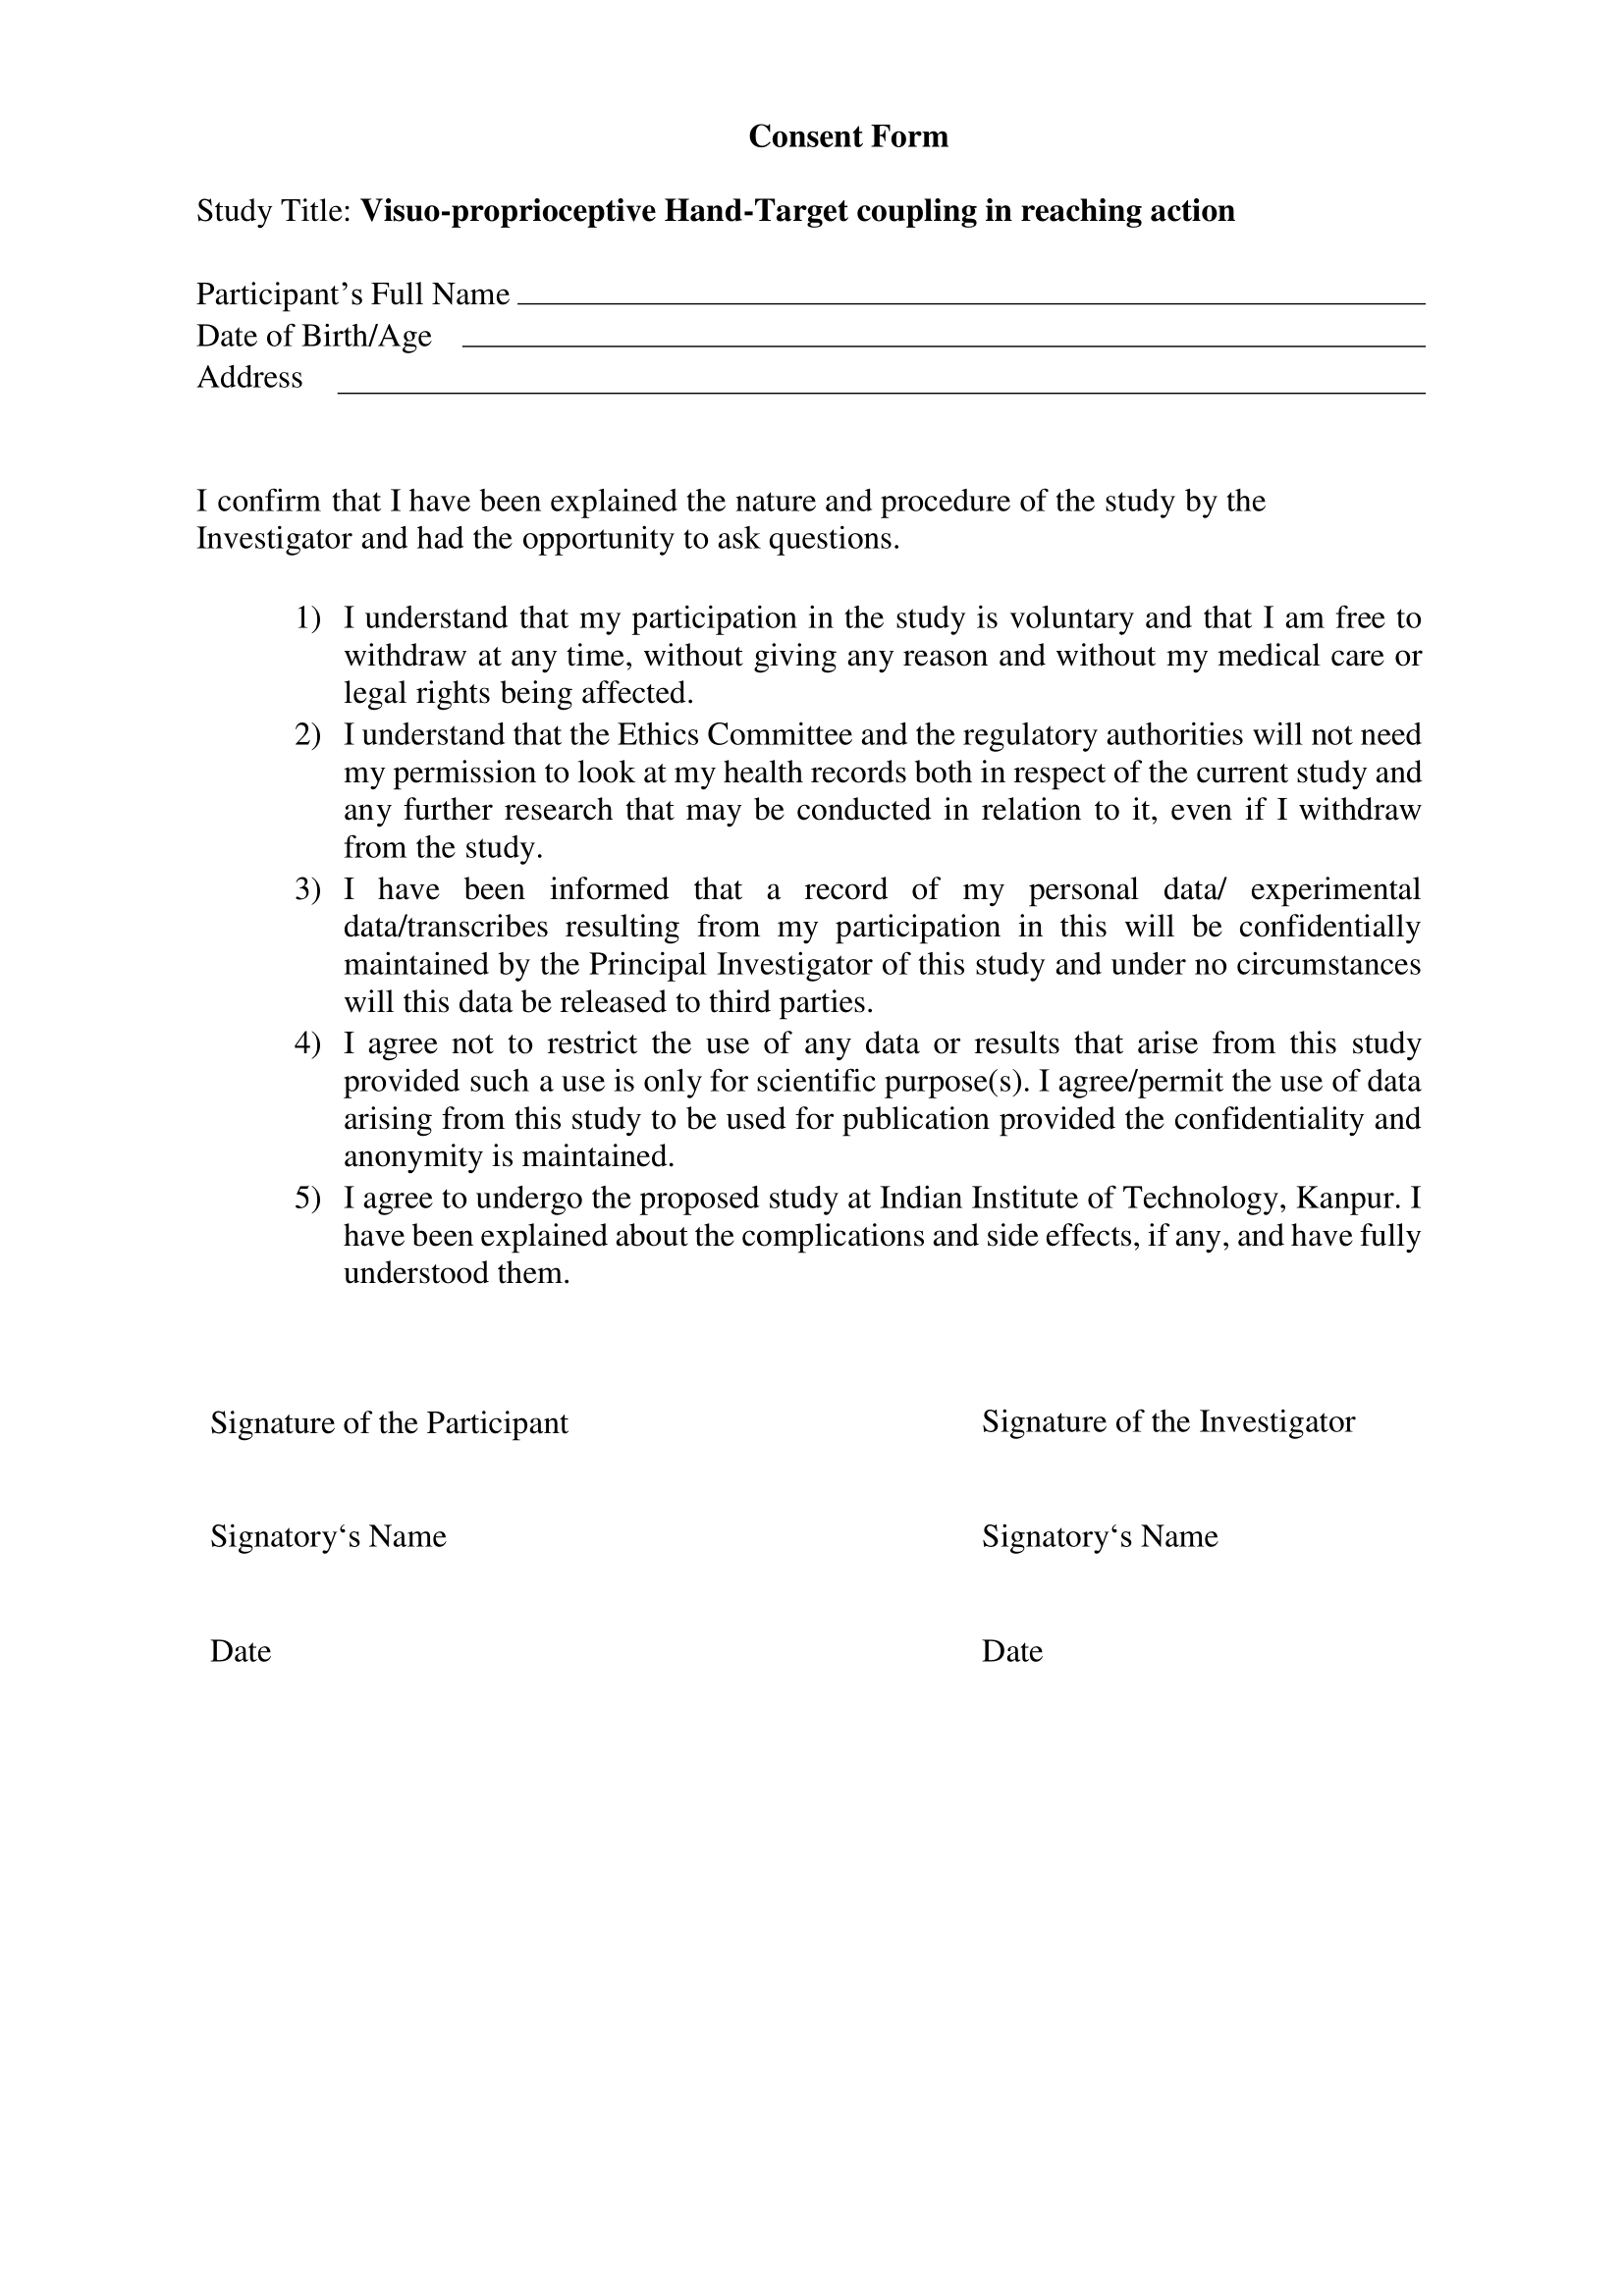
\includegraphics[width=\textwidth, keepaspectratio]{Images/admin/Consent Form- PPS Experiment-1.png}
    \caption{Consent for participation}
    \label{}
\end{figure}


\addtocontents{toc}{\vspace{2em}} % Add a gap in the Contents, for aesthetics

\backmatter


%	BIBLIOGRAPHY

%\nocite{*}
\label{Bibliography}

\lhead{\emph{Bibliography}} % Change the page header to say "Bibliography"

%\bibliographystyle{apacite} % Use the "custom" BibTeX style for formatting the Bibliography
%\setcitestyle{authoryear,open={((},close={))}} %Citation-related commands

\bibliography{Bibliography} % The references (bibliography) information are stored in the file named "Bibliography.bib"
%\bibliographystyle{apalike}

\end{document}  
